\documentclass[11pt,a4paper]{article}

\usepackage[T1]{fontenc}
\usepackage[utf8]{inputenc}
\usepackage[english]{babel}
\usepackage{lmodern}
\usepackage{amsmath,amssymb,amsfonts,mathtools}
\usepackage{booktabs}
\usepackage{geometry}
\usepackage{graphicx}
\usepackage{microtype}
\usepackage{enumitem}
\usepackage[numbers,sort&compress]{natbib}
\usepackage{caption}
\usepackage{hyperref}
\usepackage{fancyhdr}
\usepackage{xcolor}

\newcommand{\ket}[1]{\left|#1\right\rangle}
\newcommand{\bra}[1]{\left\langle#1\right|}
\newcommand{\abs}[1]{\left|#1\right|}

\geometry{margin=1in}
\setlength{\headheight}{14pt}
\hypersetup{
  hidelinks,
  pdftitle={Detailed Graph-Family Study for Open Quantum Transport},
  pdfauthor={Pedro Henrique}
}
\setlist[itemize]{leftmargin=1.4em}
\setlist[enumerate]{leftmargin=1.6em}
\captionsetup{font=small,labelfont=bf}
\pagestyle{fancy}
\fancyhf{}
\rhead{Graph-Family Transport Study}
\lhead{Open Quantum Transport}
\cfoot{\thepage}

\title{\textbf{Detailed Graph-Family Study}\\
\large Coherent and Dissipative Transport on Small Quantum Graphs}
\author{Pedro Henrique}
\date{April 2026}

\begin{document}

\maketitle
\tableofcontents
\newpage

\section{Scope}

This document studies the three graph families currently implemented in the
laboratory: chain, ring, and complete graph. The goal is not only to plot
curves, but to assign a precise physical meaning to every quantity that appears
in the simulation:
\begin{itemize}
  \item each node is a basis state $\ket{i}$, meaning ``the excitation is on site $i$'';
  \item each solid graph edge represents a coherent hopping term with amplitude $J$;
  \item the sink channel represents successful transport to the target;
  \item the loss channel represents parasitic dissipation;
  \item the population on any node is a diagonal density-matrix element;
  \item uncertainty bands come from disorder ensembles, not from measurement noise.
\end{itemize}

The guiding references are the seminal ENAQT papers
\citep{mohseni_2008, plenio_huelga_2008, rebentrost_2009, caruso_2009}, the
open-systems background texts \citep{breuer_petruccione_2007, rivas_huelga_2012},
the graph-transport review of \citet{mulken_blumen_2011}, the many-qubit
experimental benchmark \citep{maier_2019}, and the recent analytical work on
the fully connected network \citep{alterman_2024}. We also use
\citet{chin_2010,hoyer_2010,scholak_2011,novo_2016} as guardrails when
interpreting disorder, coherence, and candidate crossover lines.

\section{Model and observables}

\subsection{Hamiltonian}

The coherent transport model is a tight-binding Hamiltonian
\begin{equation}
H = \sum_i \epsilon_i \ket{i}\bra{i} + \sum_{i\neq j} J_{ij}\ket{i}\bra{j},
\end{equation}
where:
\begin{itemize}
  \item $\epsilon_i$ is the site energy of node $i$;
  \item $J_{ij}$ is the coherent coupling carried by an edge;
  \item in the present simulations the nonzero couplings have common magnitude $J$.
\end{itemize}

\subsection{Open-system dynamics}

The density matrix evolves according to the Lindblad master equation
\begin{equation}
\frac{d\rho}{dt}
= -i[H,\rho]
+ \sum_k \left(L_k\rho L_k^\dagger - \frac12\{L_k^\dagger L_k,\rho\}\right).
\end{equation}

The dissipative channels are:
\begin{itemize}
  \item local dephasing:
  \begin{equation}
  L_i^{(\phi)}=\sqrt{\gamma_\phi}\ket{i}\bra{i};
  \end{equation}
  \item sink capture from the trap site $\ket{t}$:
  \begin{equation}
  L^{(\mathrm{sink})}=\sqrt{\kappa}\ket{s}\bra{t};
  \end{equation}
  \item loss from physical nodes:
  \begin{equation}
  L_i^{(\mathrm{loss})}=\sqrt{\Gamma}\ket{\ell}\bra{i}.
  \end{equation}
\end{itemize}

\subsection{Population quantification}

The graph populations are
\begin{equation}
P_i(t)=\rho_{ii}(t),
\end{equation}
the sink population is
\begin{equation}
P_s(t)=\rho_{ss}(t),
\end{equation}
and the loss population is
\begin{equation}
P_\ell(t)=\rho_{\ell\ell}(t).
\end{equation}

The main transport observable is the sink efficiency at the final simulation time:
\begin{equation}
\eta(T)=P_s(T)=\rho_{ss}(T).
\end{equation}

This quantity is the right success metric because it distinguishes useful arrival
from generic spreading over the graph.

\subsection{Coherence and uncertainty}

The coherence measure used throughout the study is the $\ell_1$ norm of coherence,
\begin{equation}
C_{\ell_1}(\rho)=\sum_{i\neq j}\abs{\rho_{ij}}.
\end{equation}

For clean graphs, the model is deterministic, so there is no ensemble uncertainty.
For disordered graphs, the reported uncertainty bands are sample standard deviations
across static-disorder realizations generated from different seeds.

\subsection{Conditional statistical-mechanics observables}

In addition to transport efficiency and coherence, the updated collection tracks
four conditional observables evaluated on the normalized state restricted to the
physical graph nodes. This avoids confusing internal mixing with mere leakage
into the sink or the loss channel.

The conditional network purity is
\begin{equation}
\gamma(t)=\mathrm{Tr}\left[\rho_{\mathrm{net}}(t)^2\right].
\end{equation}

The conditional von Neumann entropy is
\begin{equation}
S(t)=-\mathrm{Tr}\left[\rho_{\mathrm{net}}(t)\log\rho_{\mathrm{net}}(t)\right].
\end{equation}

If $p_i(t)$ are the normalized node populations inside the graph, the Shannon
entropy of the population profile is
\begin{equation}
H_{\mathrm{pop}}(t)=-\sum_i p_i(t)\log p_i(t).
\end{equation}

The inverse participation ratio and participation ratio are
\begin{equation}
\mathrm{IPR}(t)=\sum_i p_i(t)^2,
\qquad
PR(t)=\frac{1}{\sum_i p_i(t)^2}.
\end{equation}

These observables distinguish delocalization from true mixing. Two cases can
have similar sink efficiency but reach it through very different internal
redistribution dynamics.

\subsection{Numerical correctness}

Three diagnostics are reported for every case:
\begin{enumerate}
  \item trace deviation:
  \begin{equation}
  \delta_{\mathrm{tr}}=\max_t\abs{\mathrm{Tr}\rho(t)-1};
  \end{equation}
  \item population-closure error:
  \begin{equation}
  \delta_{\mathrm{pop}}=\max_t\abs{\sum_i P_i(t)+P_s(t)+P_\ell(t)-1};
  \end{equation}
  \item minimum state eigenvalue:
  \begin{equation}
  \lambda_{\min}=\min_t \lambda_{\min}[\rho(t)].
  \end{equation}
\end{enumerate}

When these numbers stay near machine precision, the populations can be treated
as numerically reliable.

\section{Collection design}

The collection is split into two groups:
\begin{itemize}
  \item \textbf{clean cases}: zero disorder, one deterministic realization per topology;
  \item \textbf{disordered cases}: finite static disorder and an ensemble of seeds per topology.
\end{itemize}

All cases use the same dephasing scan, the same evolution time window, and the
same physical interpretation of sink and loss. This makes the comparison
meaningful across topologies.

\begin{table}[t]
\centering
\caption{Summary of the graph-family collection. Means and standard deviations are taken across disorder realizations when disorder is present.}
\begin{tabular}{lcccccc}
\toprule
Case & Group & Regime & $\eta_{\mathrm{best}}$ & $\sigma_{\eta}$ & $\gamma_{\phi}^{\mathrm{best}}$ & $C_{\ell_1}^{\mathrm{best}}$ \\
\midrule
Clean chain & clean & coherent & 0.812 & 0.000 & 0.000 & 0.734 \\
Clean ring & clean & intermediate & 0.732 & 0.000 & 0.800 & 0.287 \\
Clean complete & clean & intermediate & 0.714 & 0.000 & 3.200 & 0.144 \\
Disordered chain & disordered & intermediate & 0.746 & 0.034 & 0.100 & 0.700 \\
Disordered ring & disordered & intermediate & 0.732 & 0.016 & 0.800 & 0.285 \\
Disordered complete & disordered & intermediate & 0.716 & 0.010 & 3.200 & 0.143 \\
\bottomrule
\end{tabular}
\end{table}


\section{Graph schematics}

\begin{figure}[t]
  \centering
  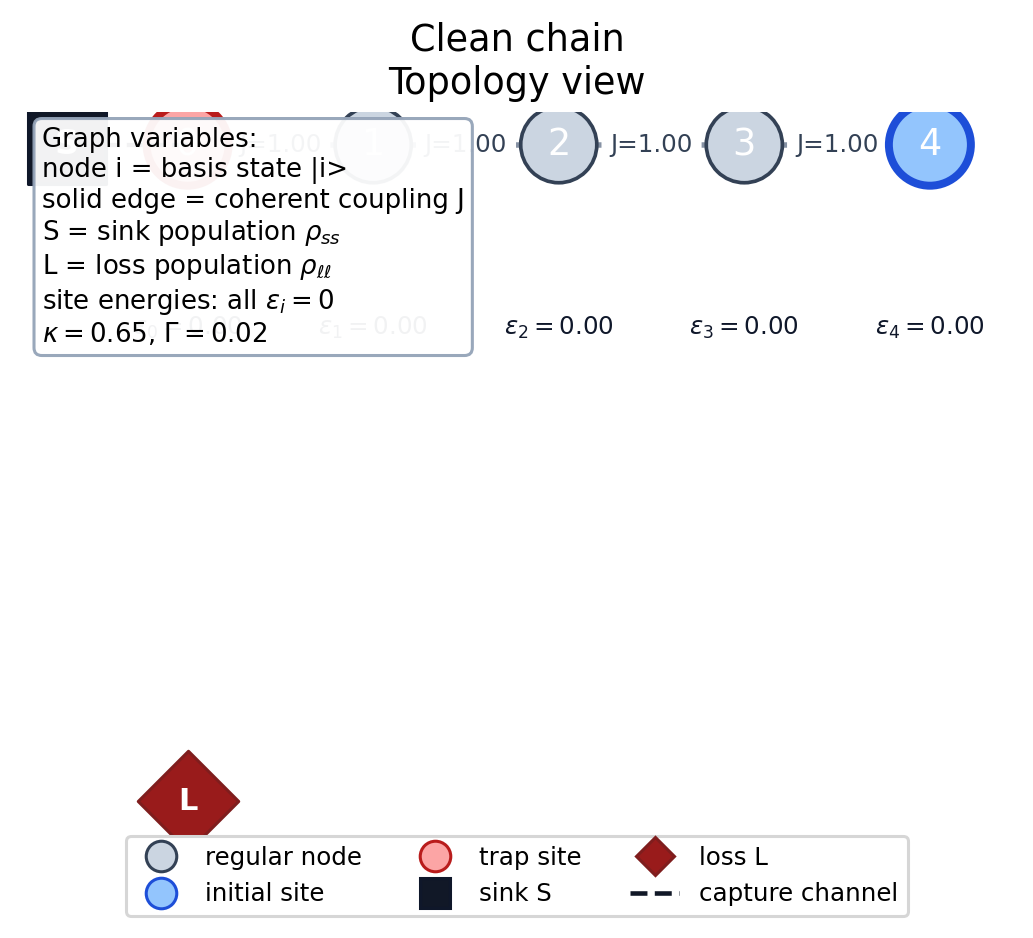
\includegraphics[width=0.32\textwidth]{../../outputs/transport_networks/graph_collection/latest/figures/clean_chain_topology.png}
  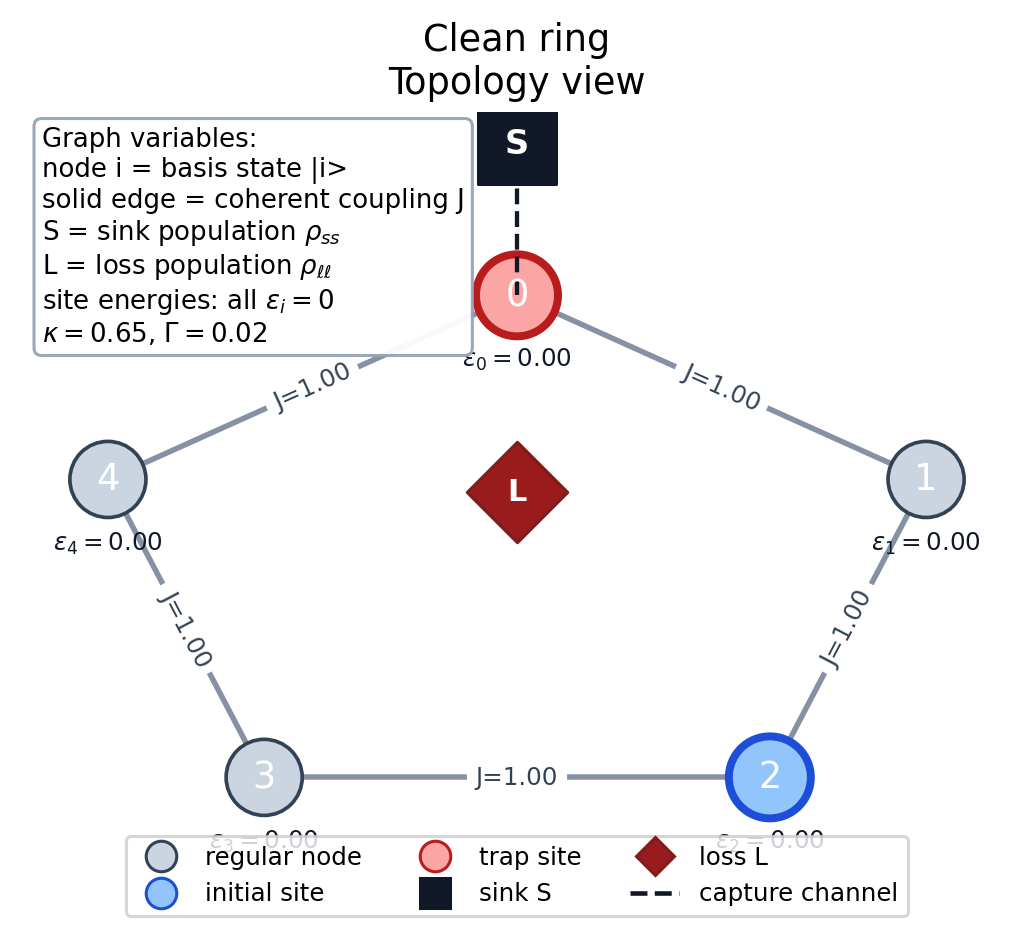
\includegraphics[width=0.32\textwidth]{../../outputs/transport_networks/graph_collection/latest/figures/clean_ring_topology.png}
  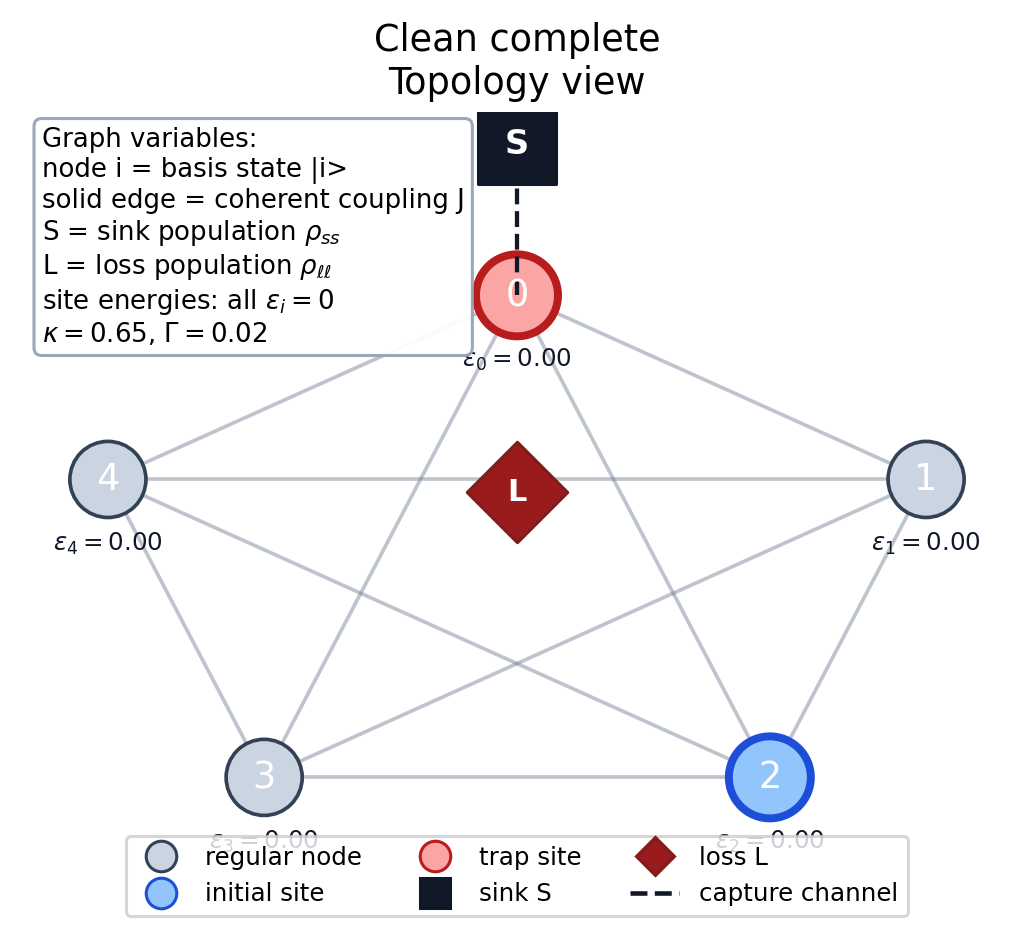
\includegraphics[width=0.32\textwidth]{../../outputs/transport_networks/graph_collection/latest/figures/clean_complete_topology.png}
  \caption{Representative clean graph layouts. Every solid edge carries the coherent hopping amplitude $J$. The blue node is the initial site, the red node is the trap site, the square $S$ is the sink, and the diamond $L$ is the loss channel. Numbers under nodes are site energies $\epsilon_i$.}
\end{figure}

\begin{figure}[t]
  \centering
  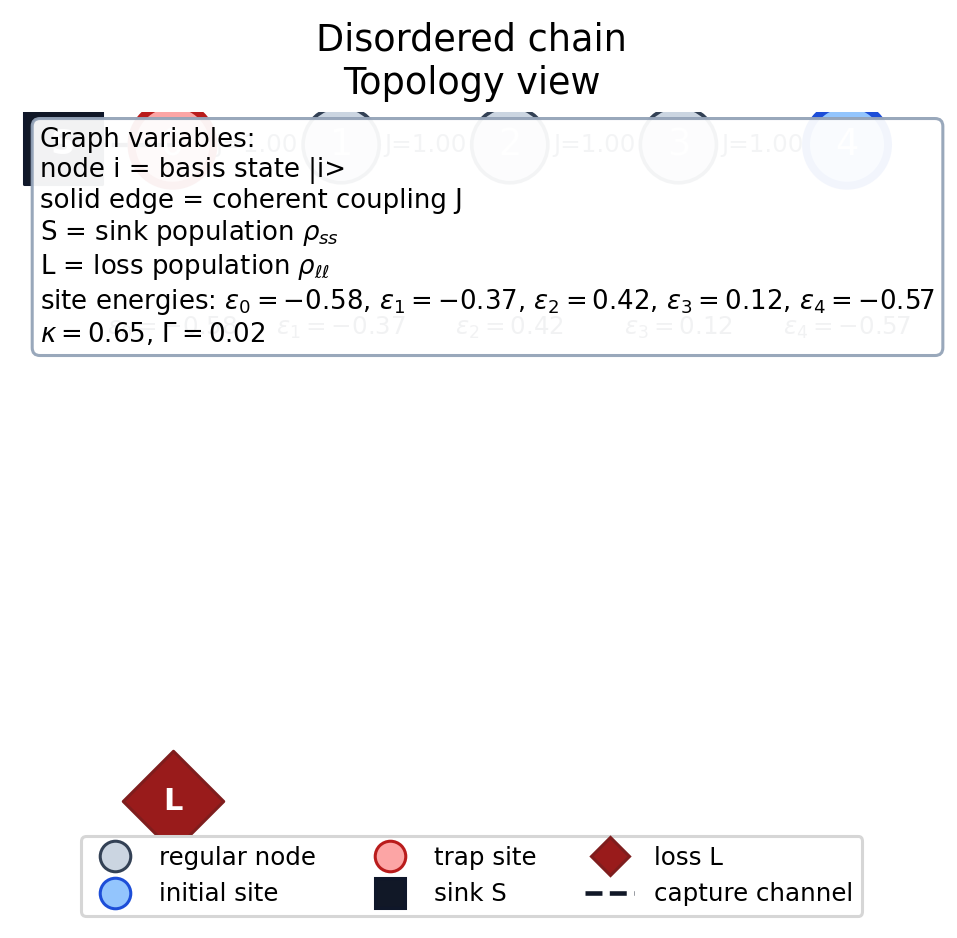
\includegraphics[width=0.32\textwidth]{../../outputs/transport_networks/graph_collection/latest/figures/disordered_chain_topology.png}
  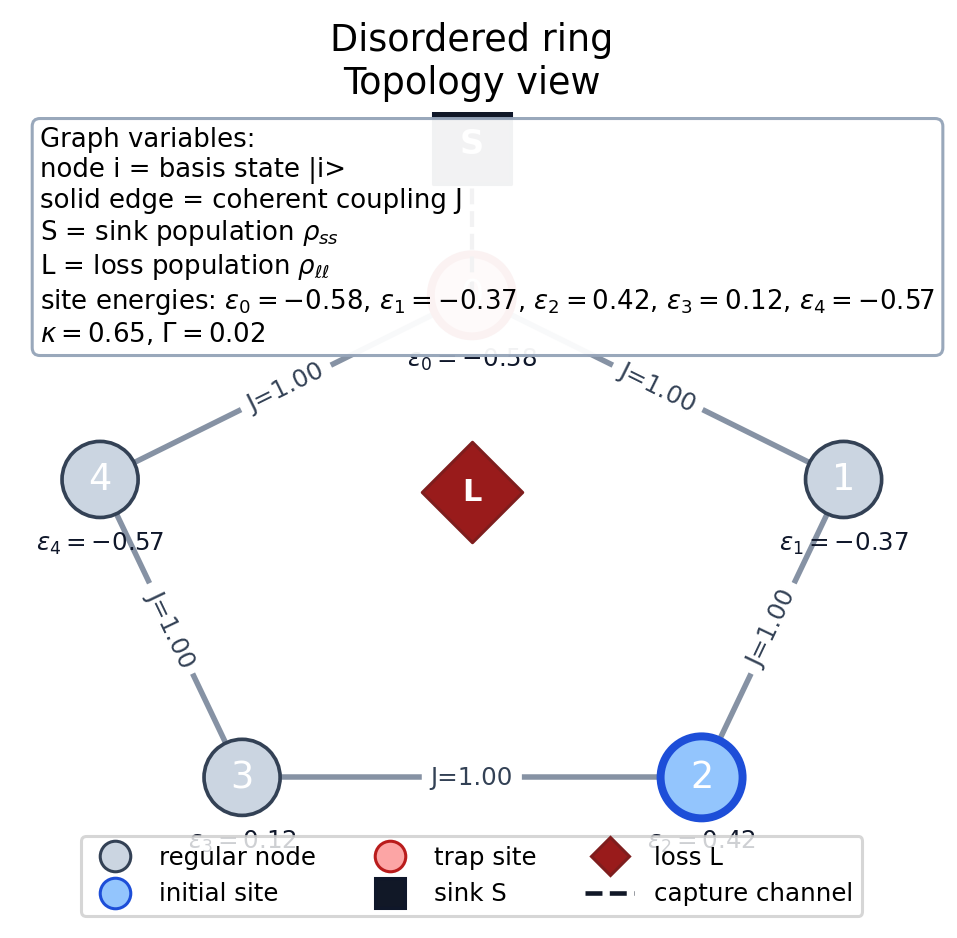
\includegraphics[width=0.32\textwidth]{../../outputs/transport_networks/graph_collection/latest/figures/disordered_ring_topology.png}
  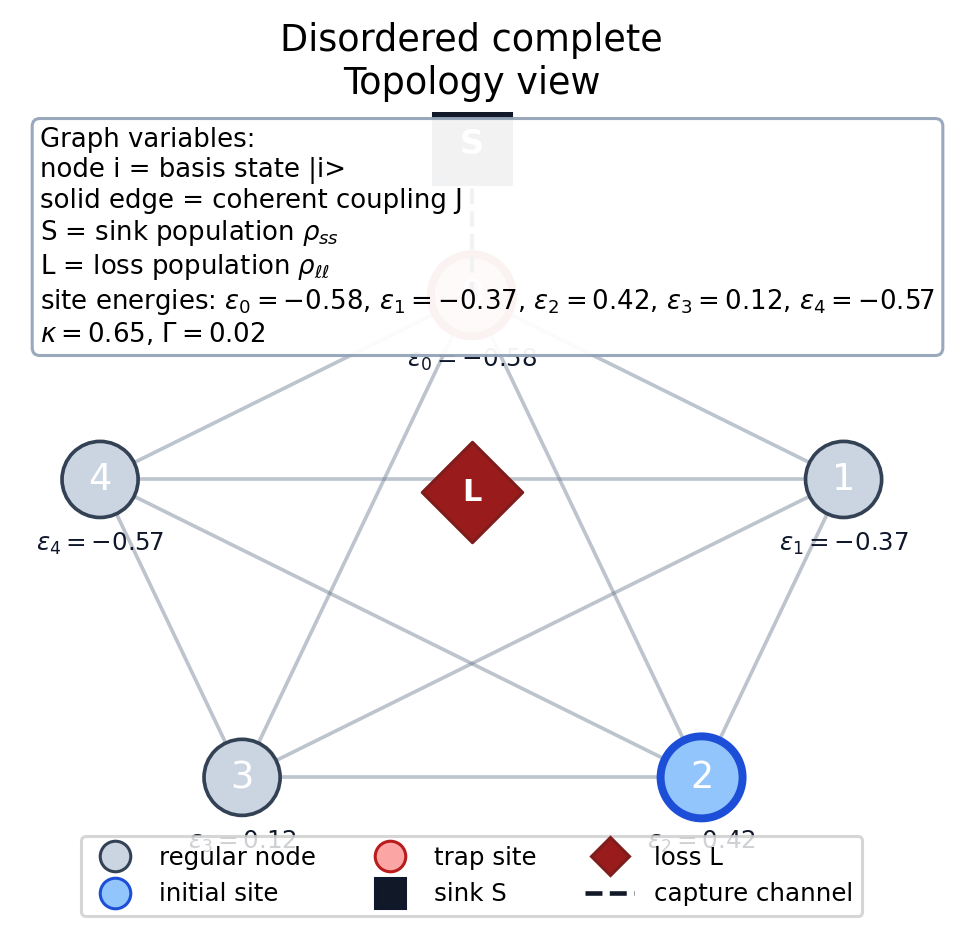
\includegraphics[width=0.32\textwidth]{../../outputs/transport_networks/graph_collection/latest/figures/disordered_complete_topology.png}
  \caption{Representative disordered graph layouts. The graph topology is unchanged, but the on-site energies $\epsilon_i$ now vary from node to node. The uncertainty analysis below quantifies how this disorder spread affects transport.}
\end{figure}

\section{Clean cases: pairwise analysis}

\begin{figure}[t]
  \centering
  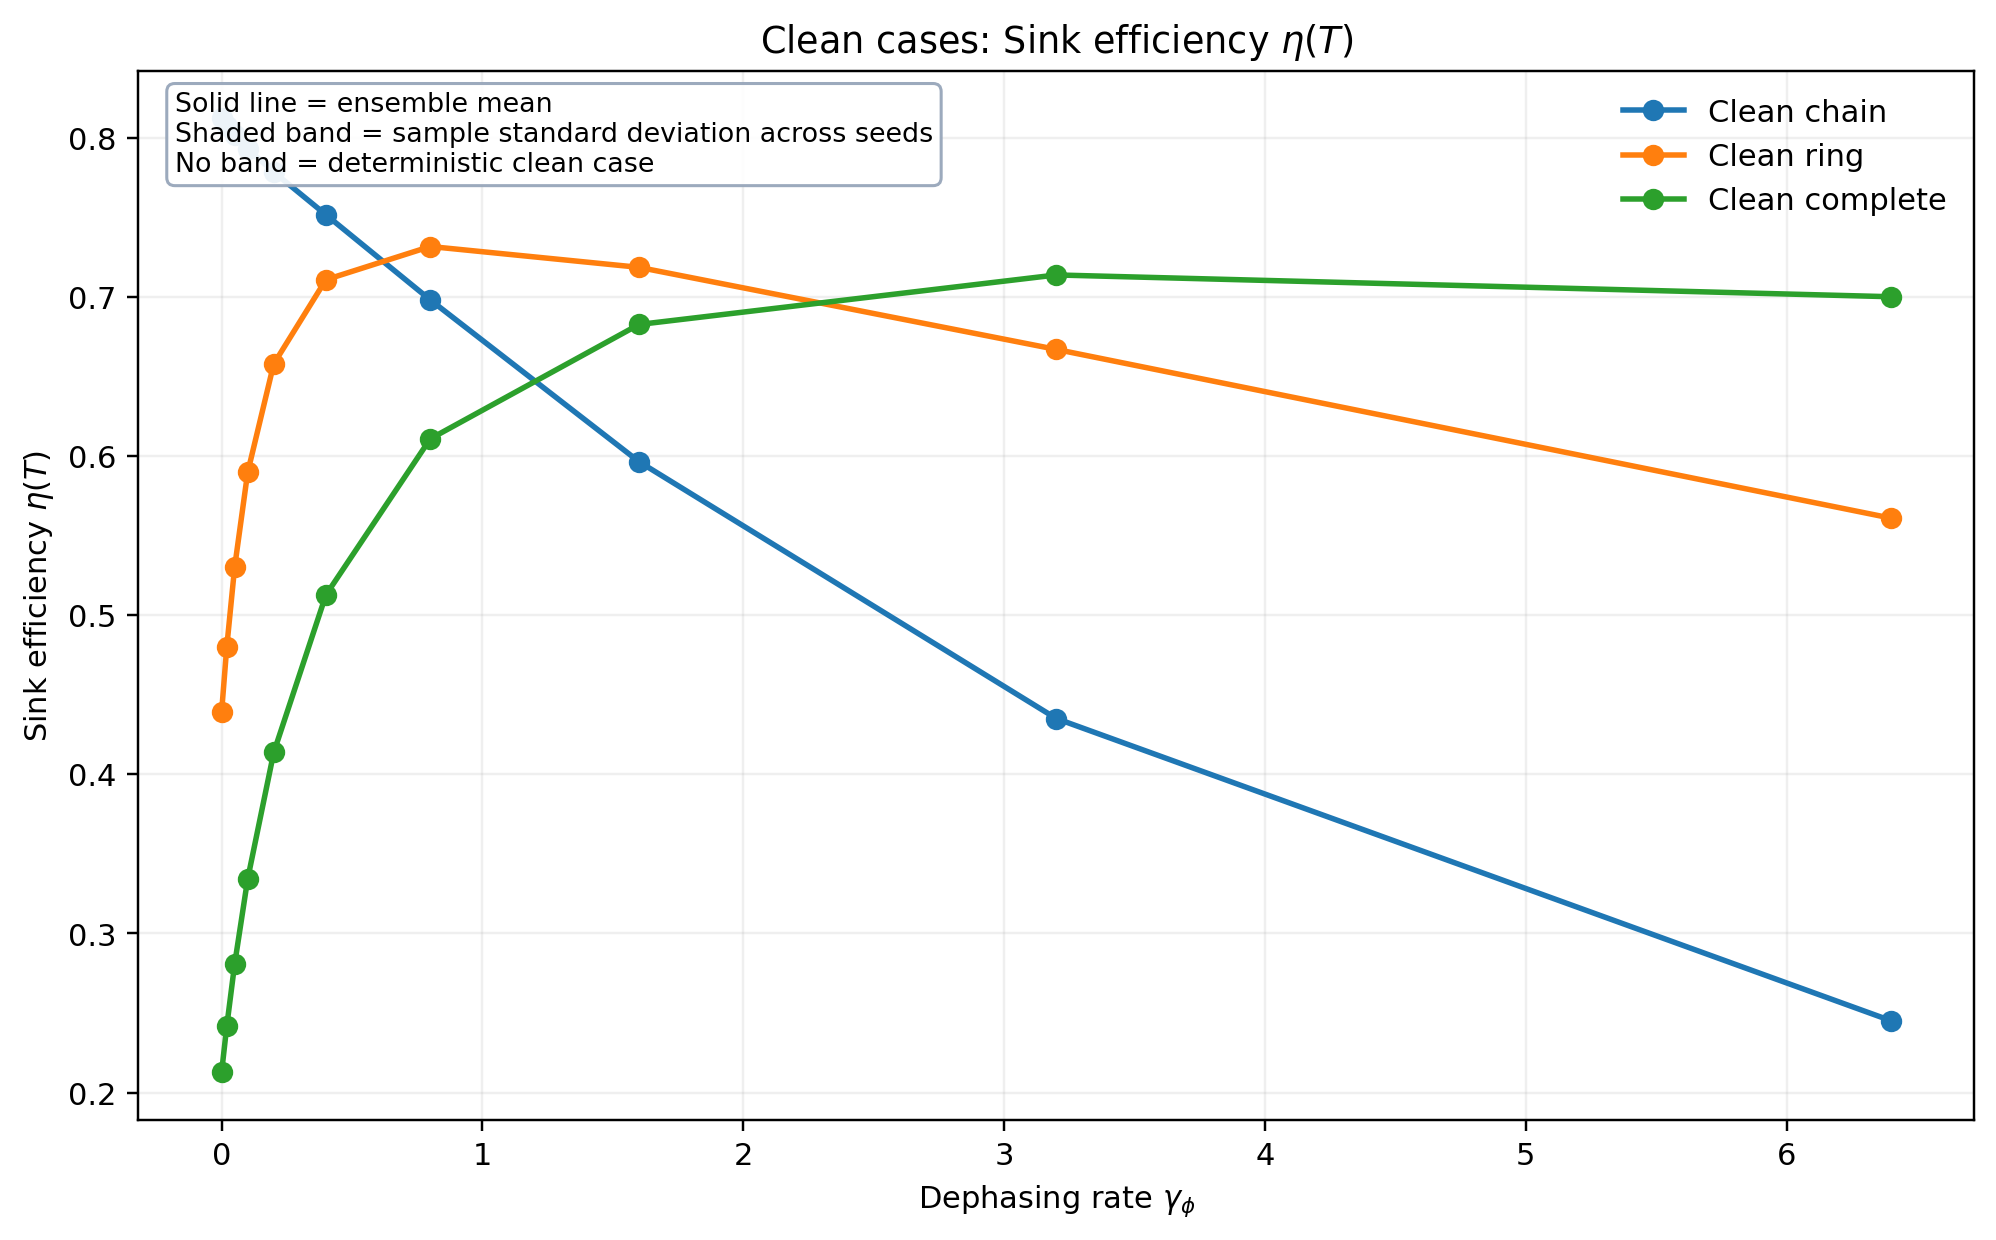
\includegraphics[width=0.78\textwidth]{../../outputs/transport_networks/graph_collection/latest/figures/clean_sink_efficiency.png}
  \caption{Mean sink efficiency versus dephasing rate for the clean graph family. The horizontal axis is the dephasing rate $\gamma_\phi$ in the same units as $J$, and the vertical axis is the final sink population $\eta(T)=\rho_{ss}(T)$. No uncertainty band is shown because these cases are deterministic.}
\end{figure}

\begin{figure}[t]
  \centering
  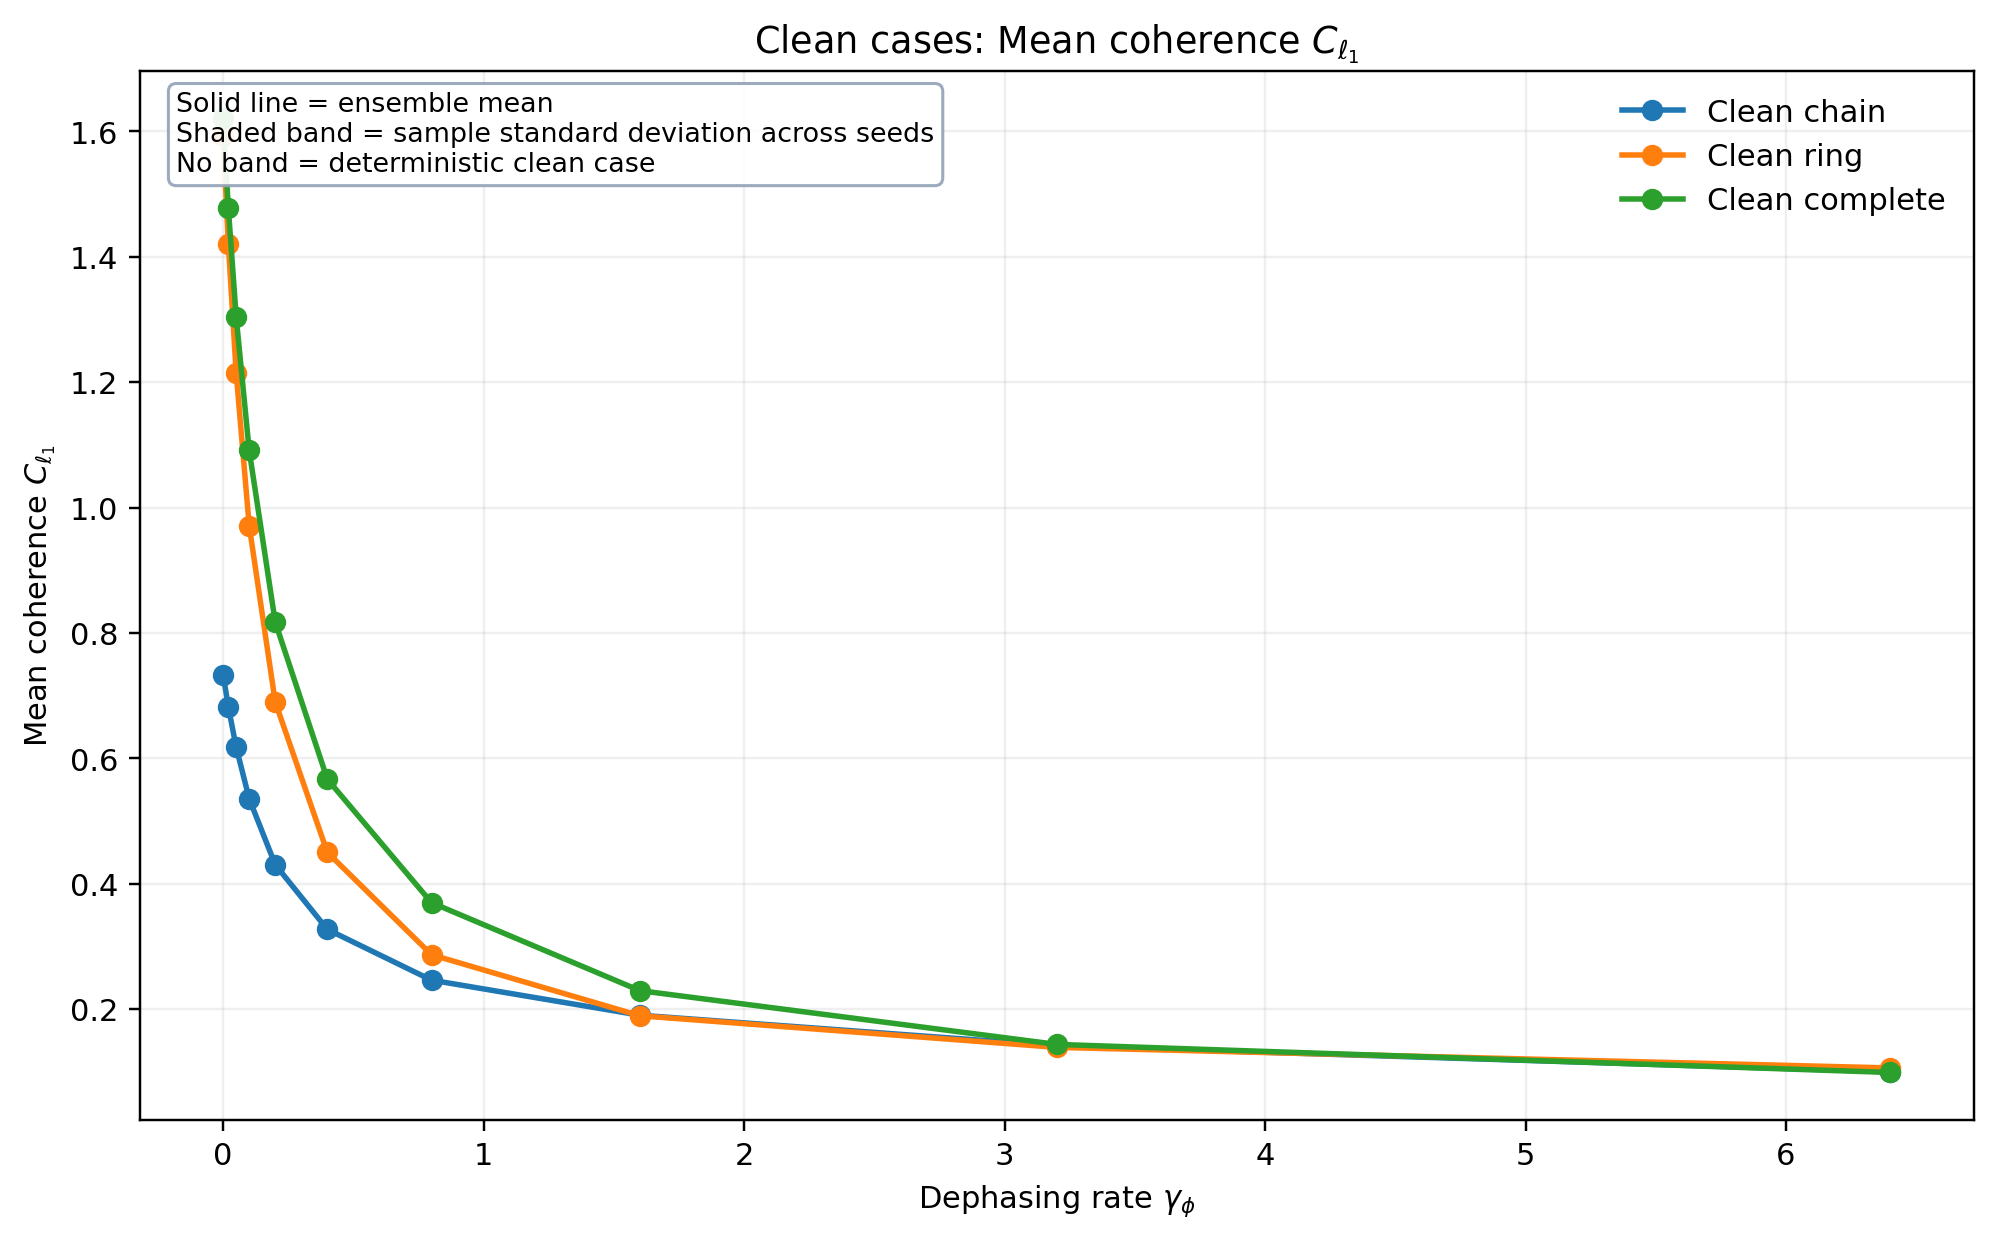
\includegraphics[width=0.78\textwidth]{../../outputs/transport_networks/graph_collection/latest/figures/clean_coherence.png}
  \caption{Mean coherence versus dephasing rate for the clean graph family. The vertical axis is $C_{\ell_1}$, the sum of the absolute values of off-diagonal density-matrix elements in the node basis. Larger values mean more phase coherence survives.}
\end{figure}

\begin{figure}[t]
  \centering
  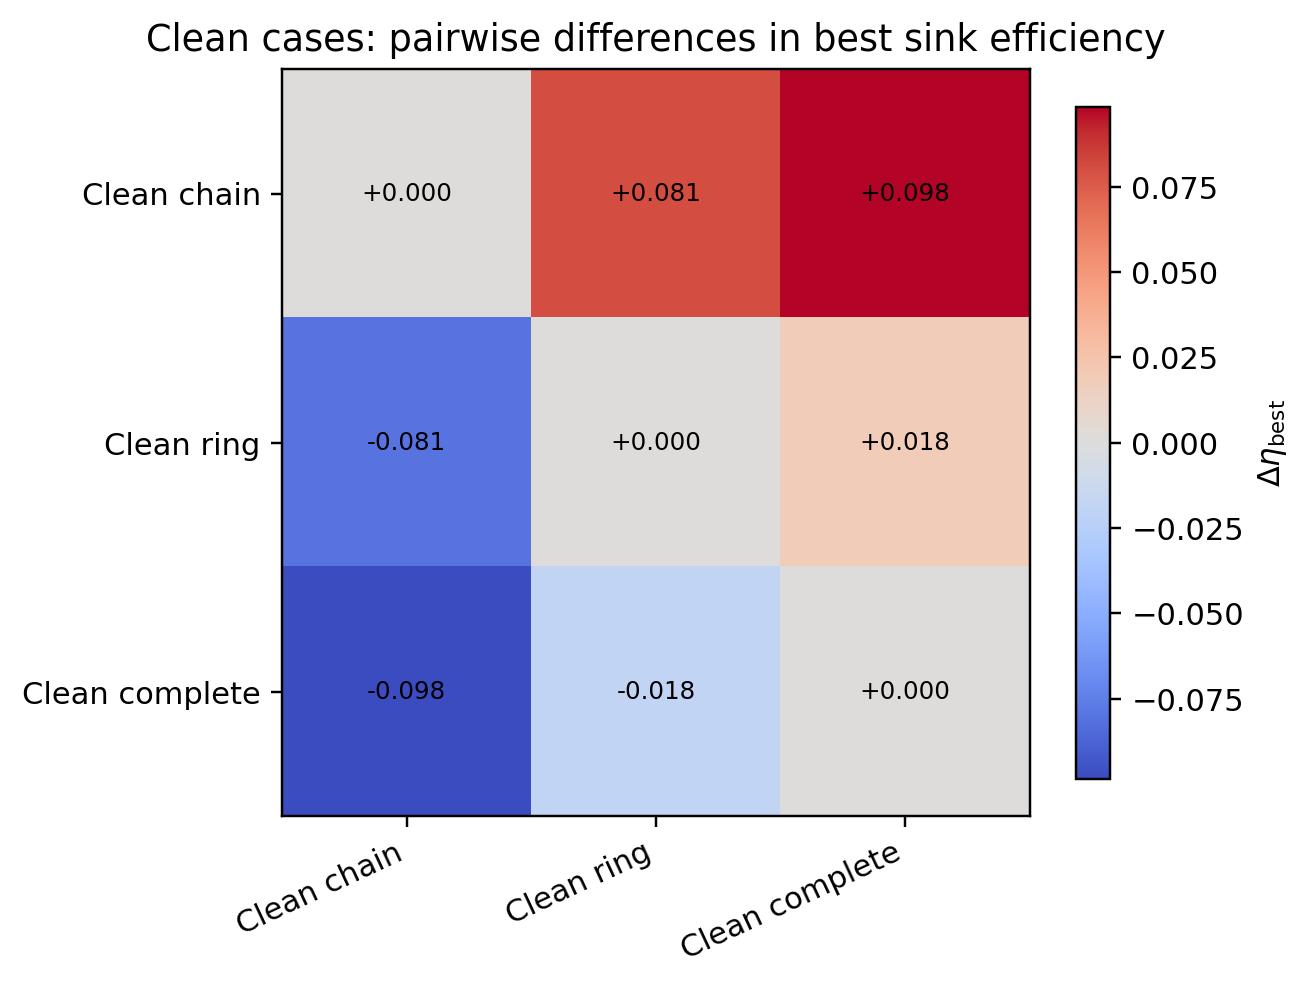
\includegraphics[width=0.62\textwidth]{../../outputs/transport_networks/graph_collection/latest/figures/clean_pairwise_eta_best.png}
  \caption{Pairwise differences in the best sink efficiency for the clean cases. Entry $(i,j)$ equals $\eta_{\mathrm{best},i}-\eta_{\mathrm{best},j}$, so positive values mean row $i$ outperforms column $j$.}
\end{figure}

The clean collection shows three distinct behaviors:
\begin{itemize}
  \item the chain performs best in the coherent limit;
  \item the ring benefits from a moderate amount of dephasing;
  \item the complete graph requires stronger dephasing to reach its optimum.
\end{itemize}

This is physically consistent with the literature: dephasing can remove
destructive interference or dark-state bottlenecks, but whether that helps
depends strongly on topology \citep{plenio_huelga_2008, rebentrost_2009,
alterman_2024}.

\begin{figure}[t]
  \centering
  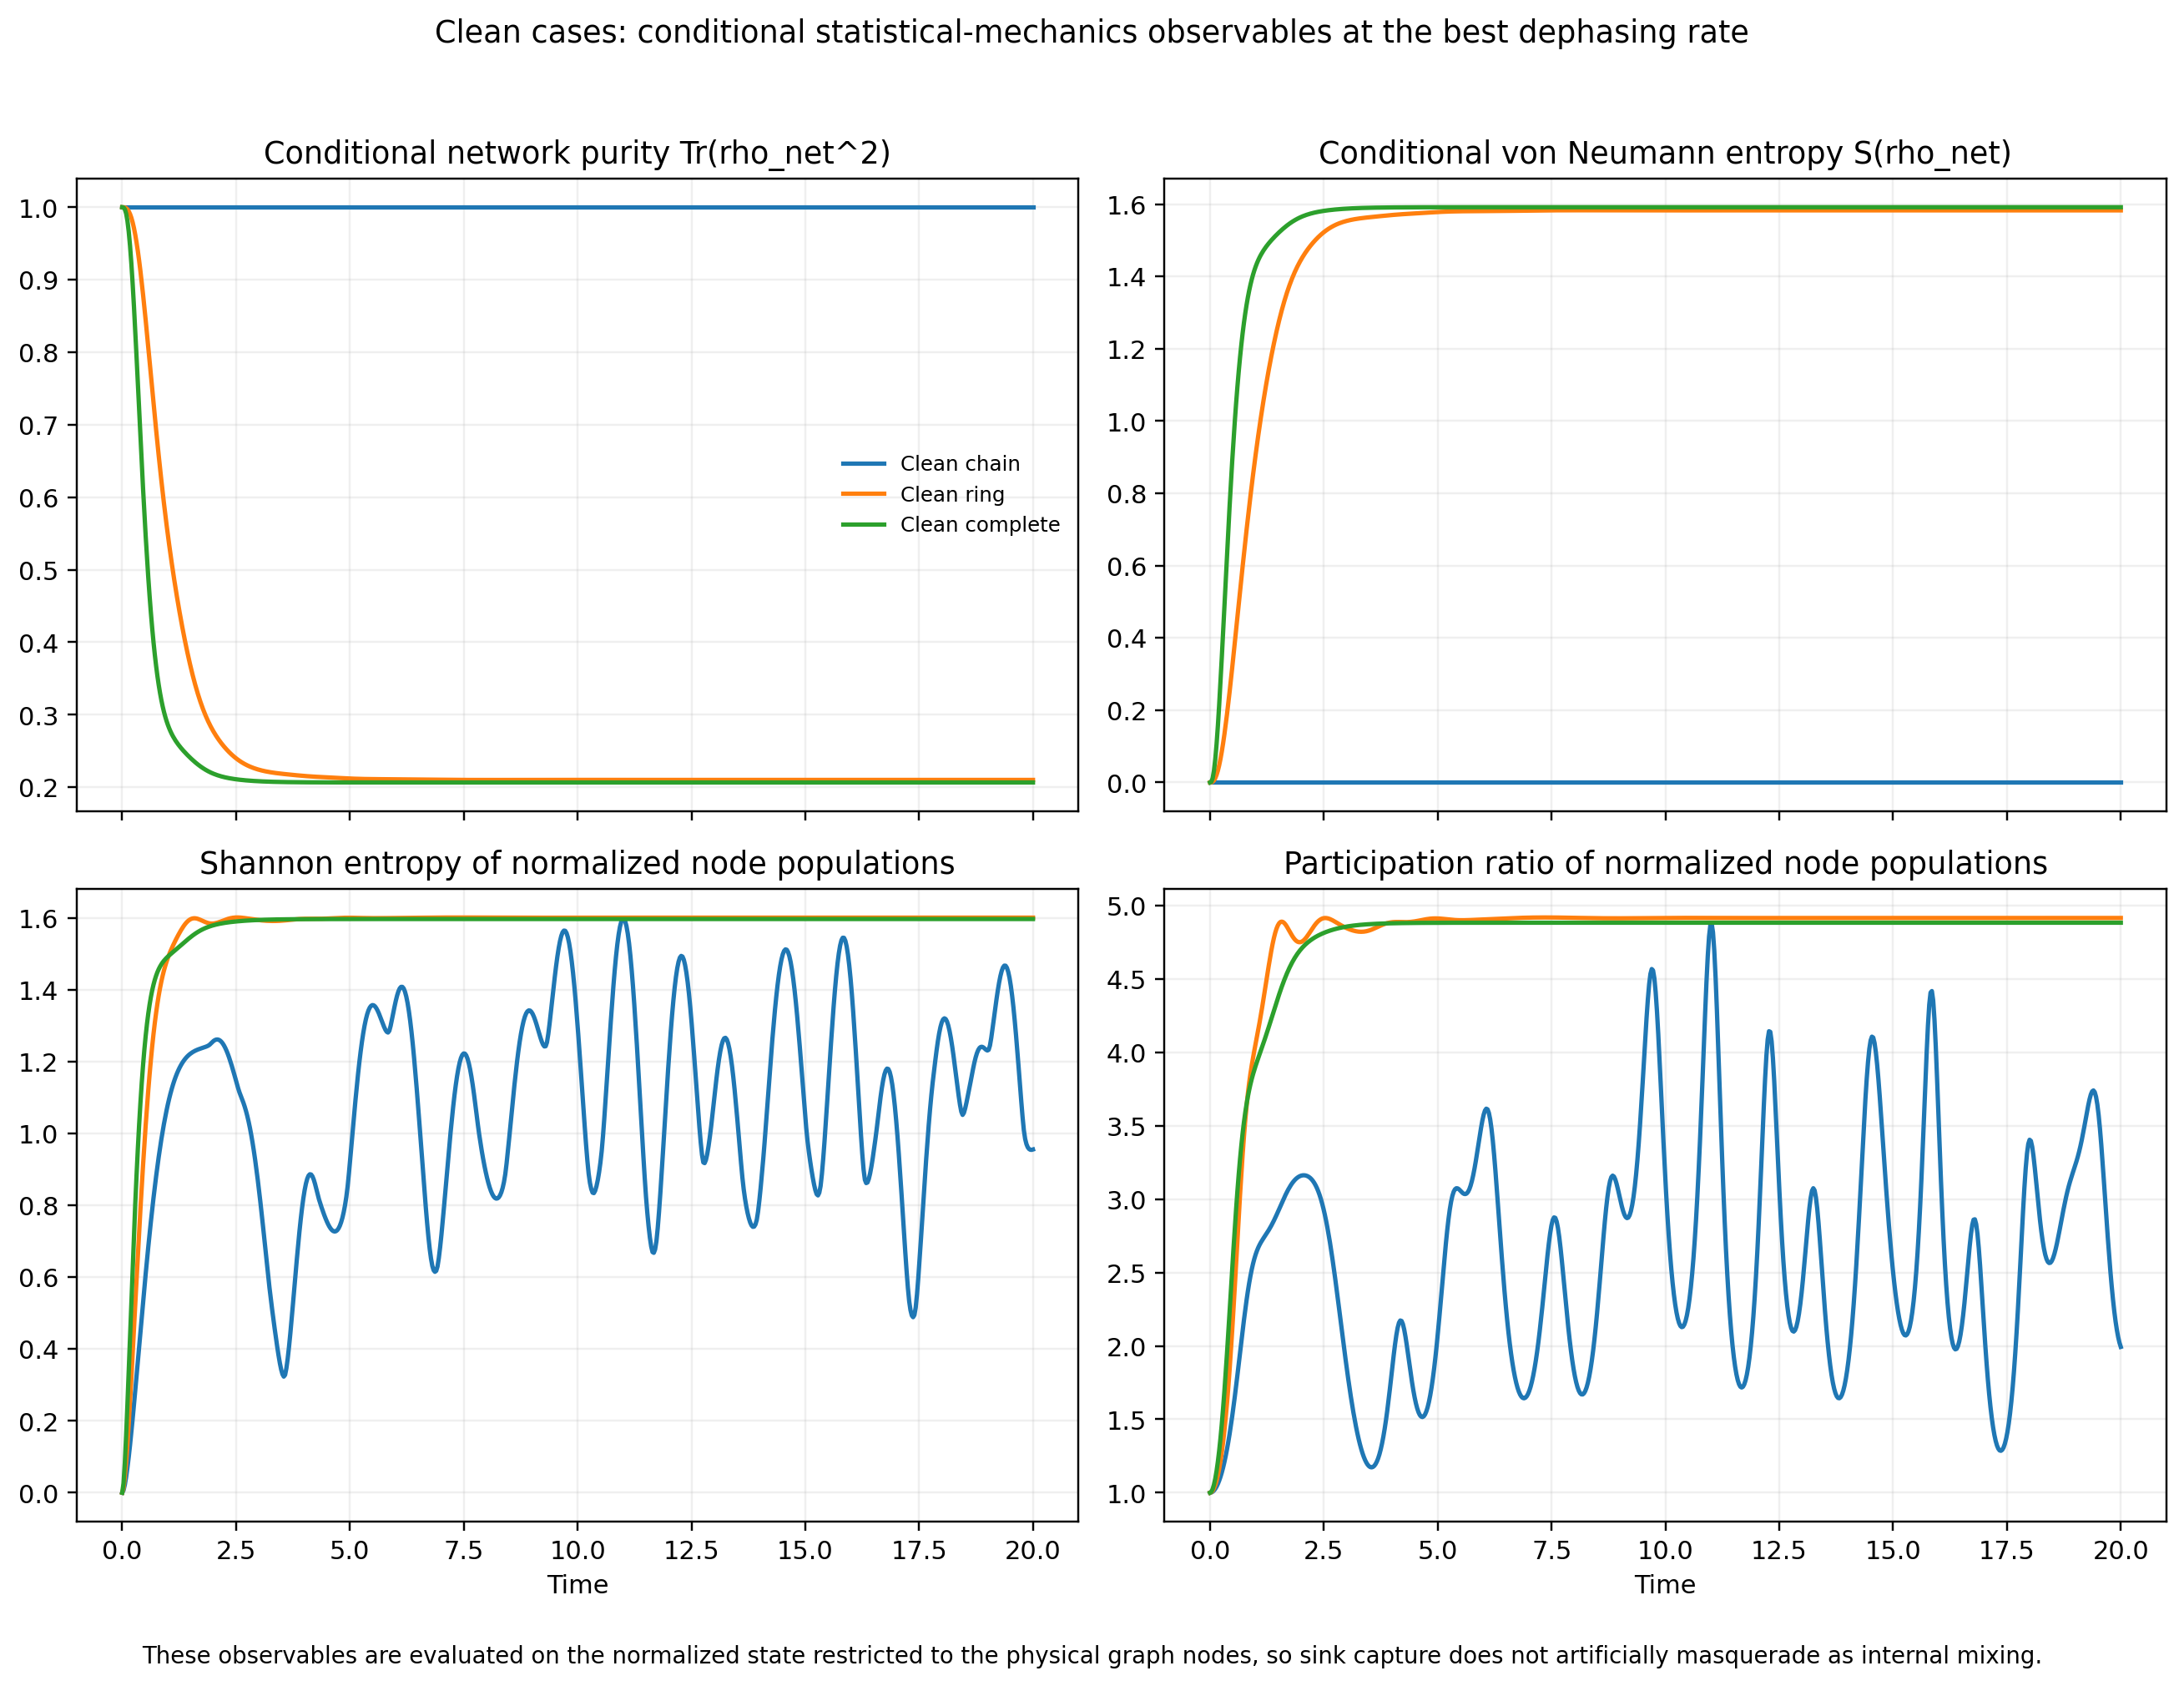
\includegraphics[width=0.84\textwidth]{../../outputs/transport_networks/graph_collection/latest/figures/clean_statmech_observables.png}
  \caption{Conditional statistical-mechanics observables for the clean family at the best dephasing rate of each case. The quantities are computed on the normalized state restricted to the physical graph nodes, so they quantify internal redistribution rather than sink capture.}
\end{figure}

\section{Disordered cases: pairwise analysis}

\begin{figure}[t]
  \centering
  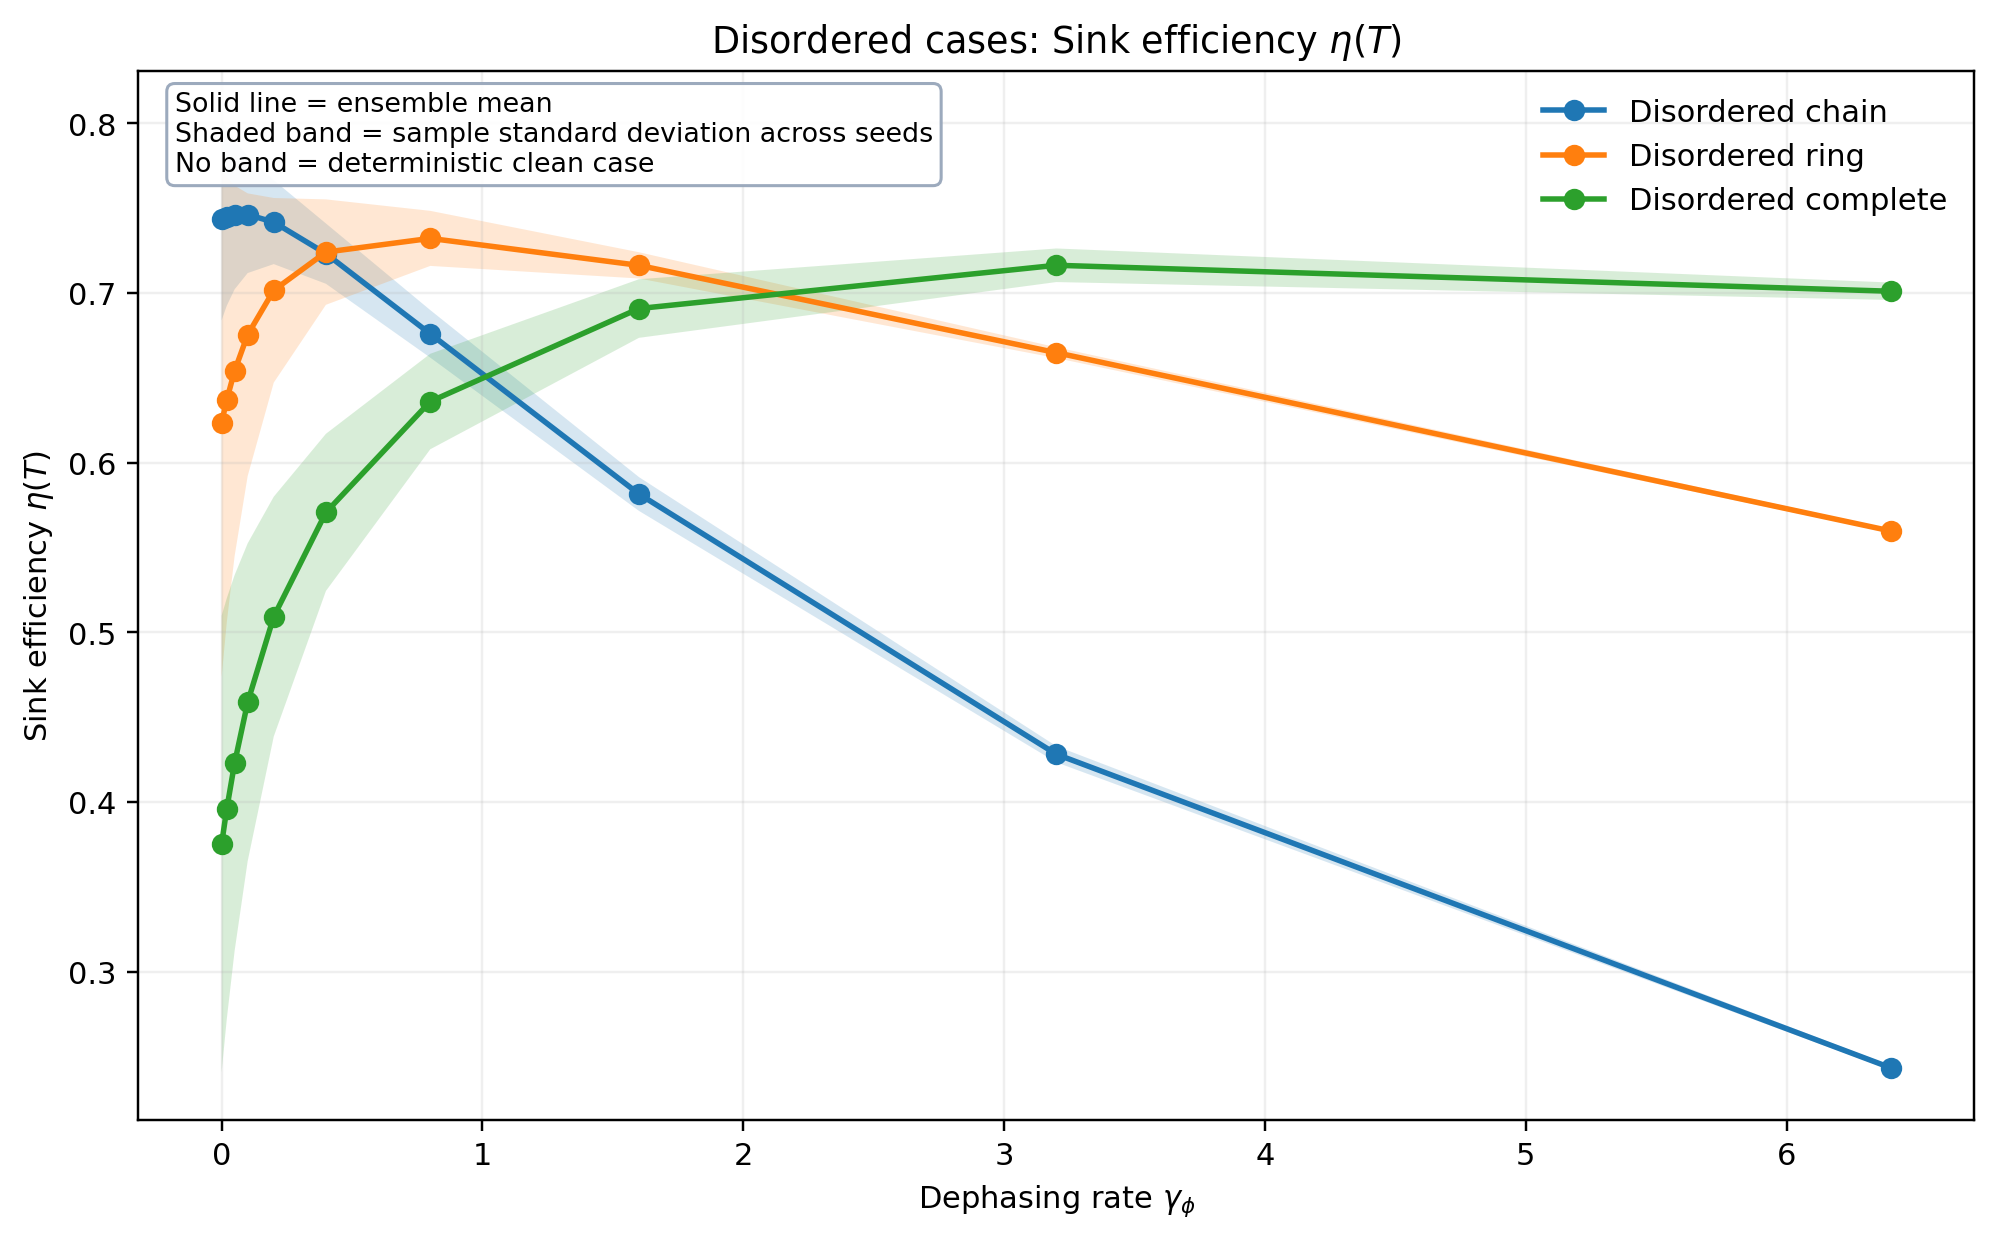
\includegraphics[width=0.78\textwidth]{../../outputs/transport_networks/graph_collection/latest/figures/disordered_sink_efficiency.png}
  \caption{Mean sink efficiency versus dephasing rate for the disordered graph family. The shaded bands are sample standard deviations across static-disorder realizations. They measure sensitivity to disorder, not shot noise or experimental uncertainty.}
\end{figure}

\begin{figure}[t]
  \centering
  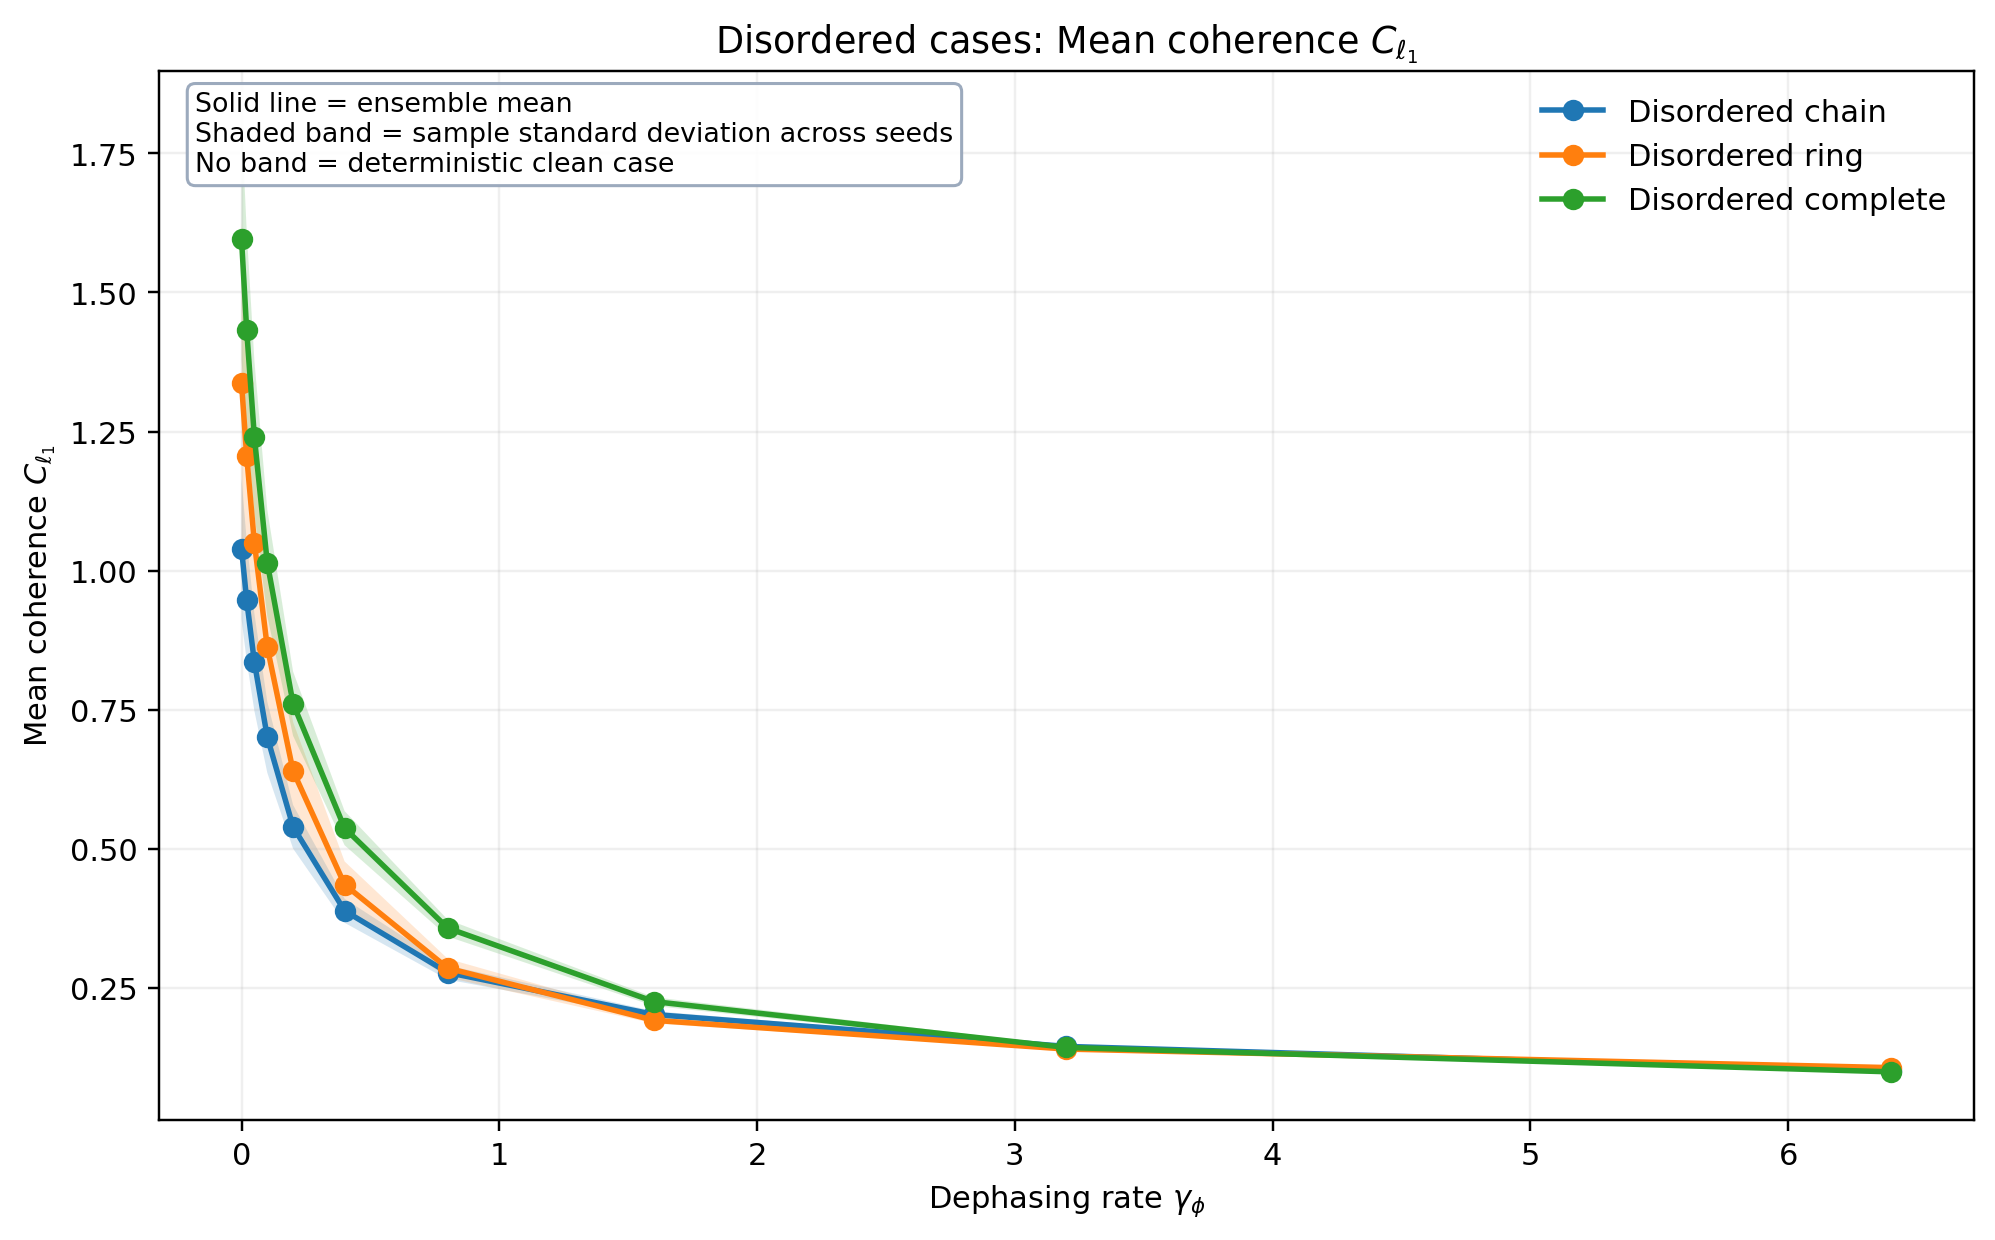
\includegraphics[width=0.78\textwidth]{../../outputs/transport_networks/graph_collection/latest/figures/disordered_coherence.png}
  \caption{Mean coherence versus dephasing rate for the disordered graph family. The same ensemble averaging is used as in the sink-efficiency plot. The disorder broadens the response, especially in the ring case.}
\end{figure}

\begin{figure}[t]
  \centering
  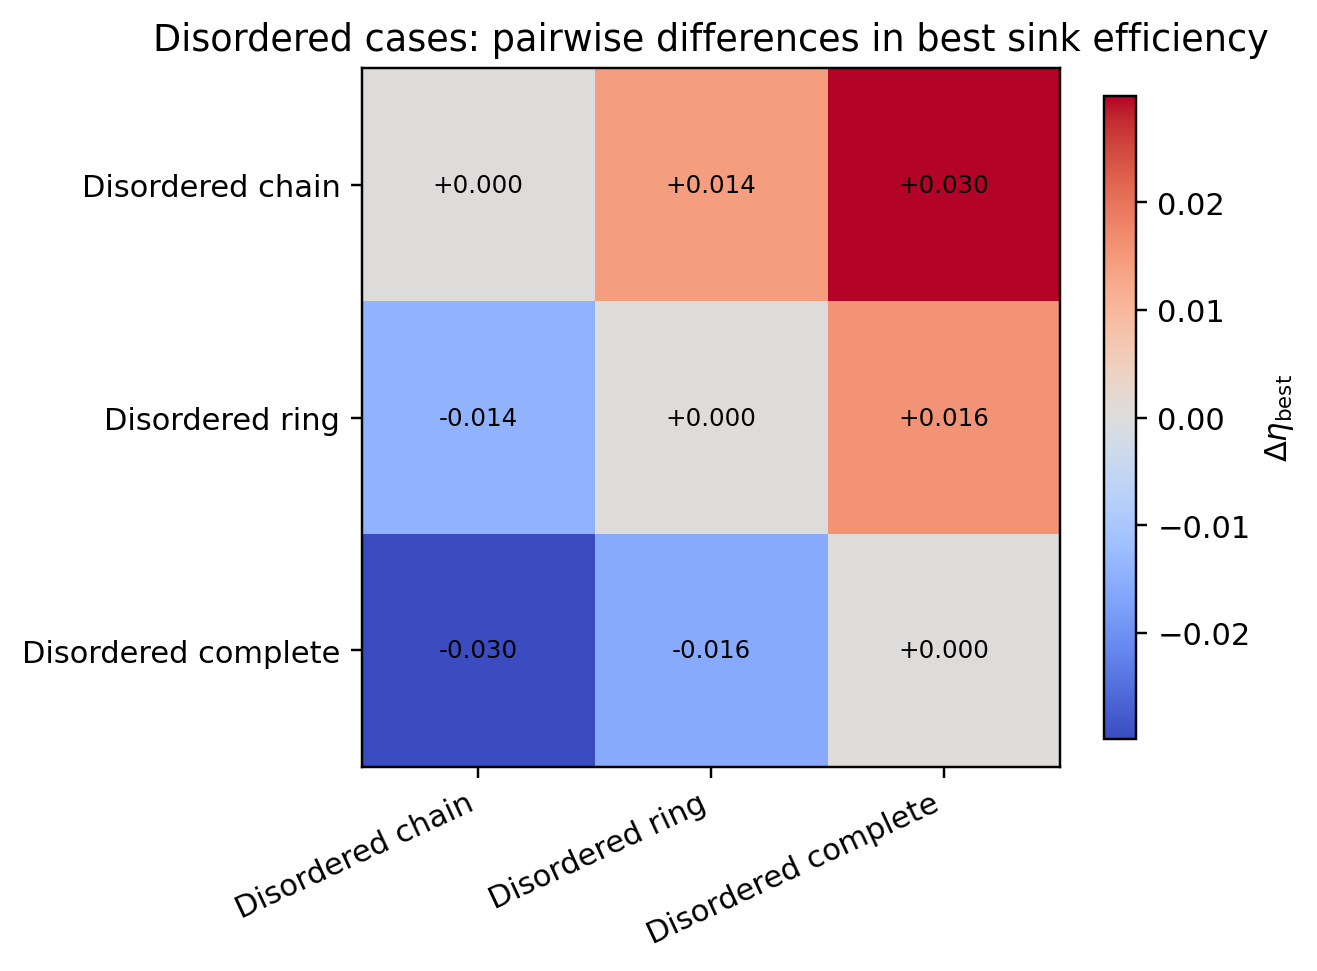
\includegraphics[width=0.62\textwidth]{../../outputs/transport_networks/graph_collection/latest/figures/disordered_pairwise_eta_best.png}
  \caption{Pairwise differences in the best sink efficiency for the disordered cases. Compared with the clean family, the pairwise differences are smaller, which means disorder compresses the performance gap between topologies.}
\end{figure}

The disordered collection changes the ranking slightly:
\begin{itemize}
  \item the ring becomes the best mean performer in the present ensemble;
  \item the chain remains competitive but shifts to a mildly dissipative optimum;
  \item the complete graph still prefers stronger dephasing than the other two.
\end{itemize}

The wide uncertainty band in the disordered ring case is important. It means the
average is good, but the response is more realization-dependent. That is a real
physical statement about sensitivity to static disorder.

\begin{figure}[t]
  \centering
  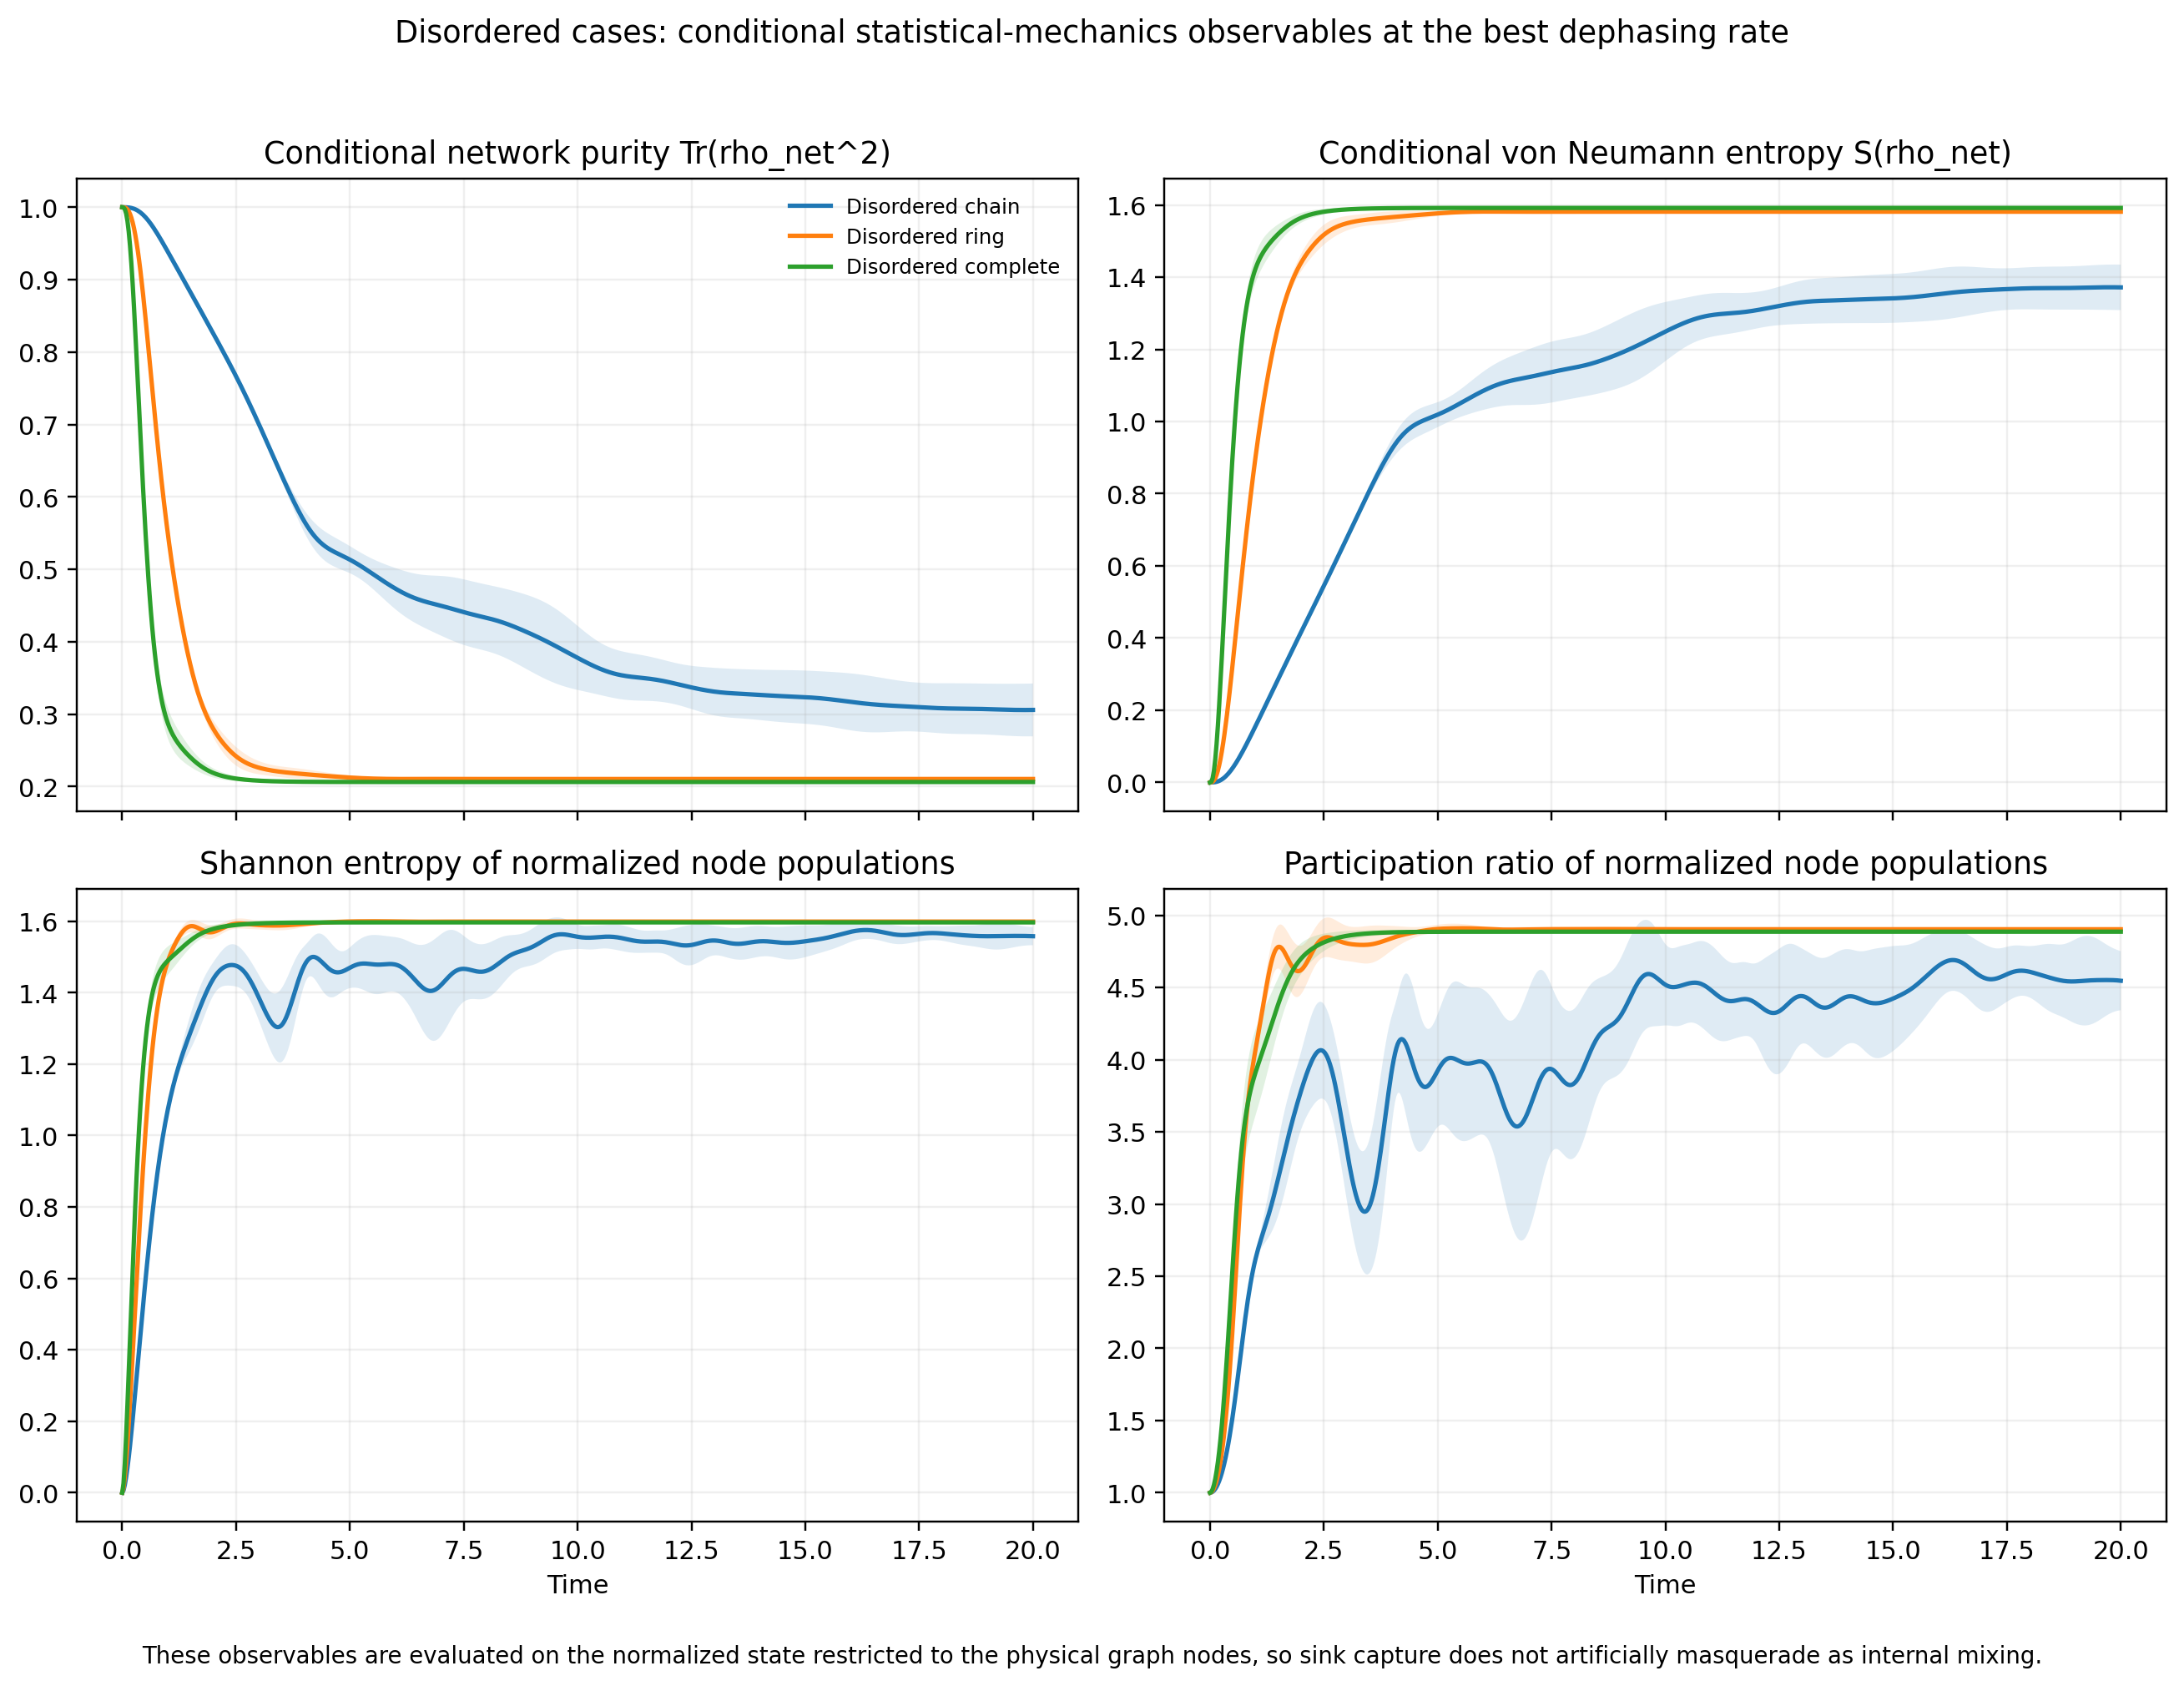
\includegraphics[width=0.84\textwidth]{../../outputs/transport_networks/graph_collection/latest/figures/disordered_statmech_observables.png}
  \caption{Conditional statistical-mechanics observables for the disordered family at the best dephasing rate of each case. Because the disorder ensemble is now larger, the bands report a more meaningful spread across realizations than in the initial pilot runs.}
\end{figure}

\section{Population-dynamics reading}

\begin{figure}[t]
  \centering
  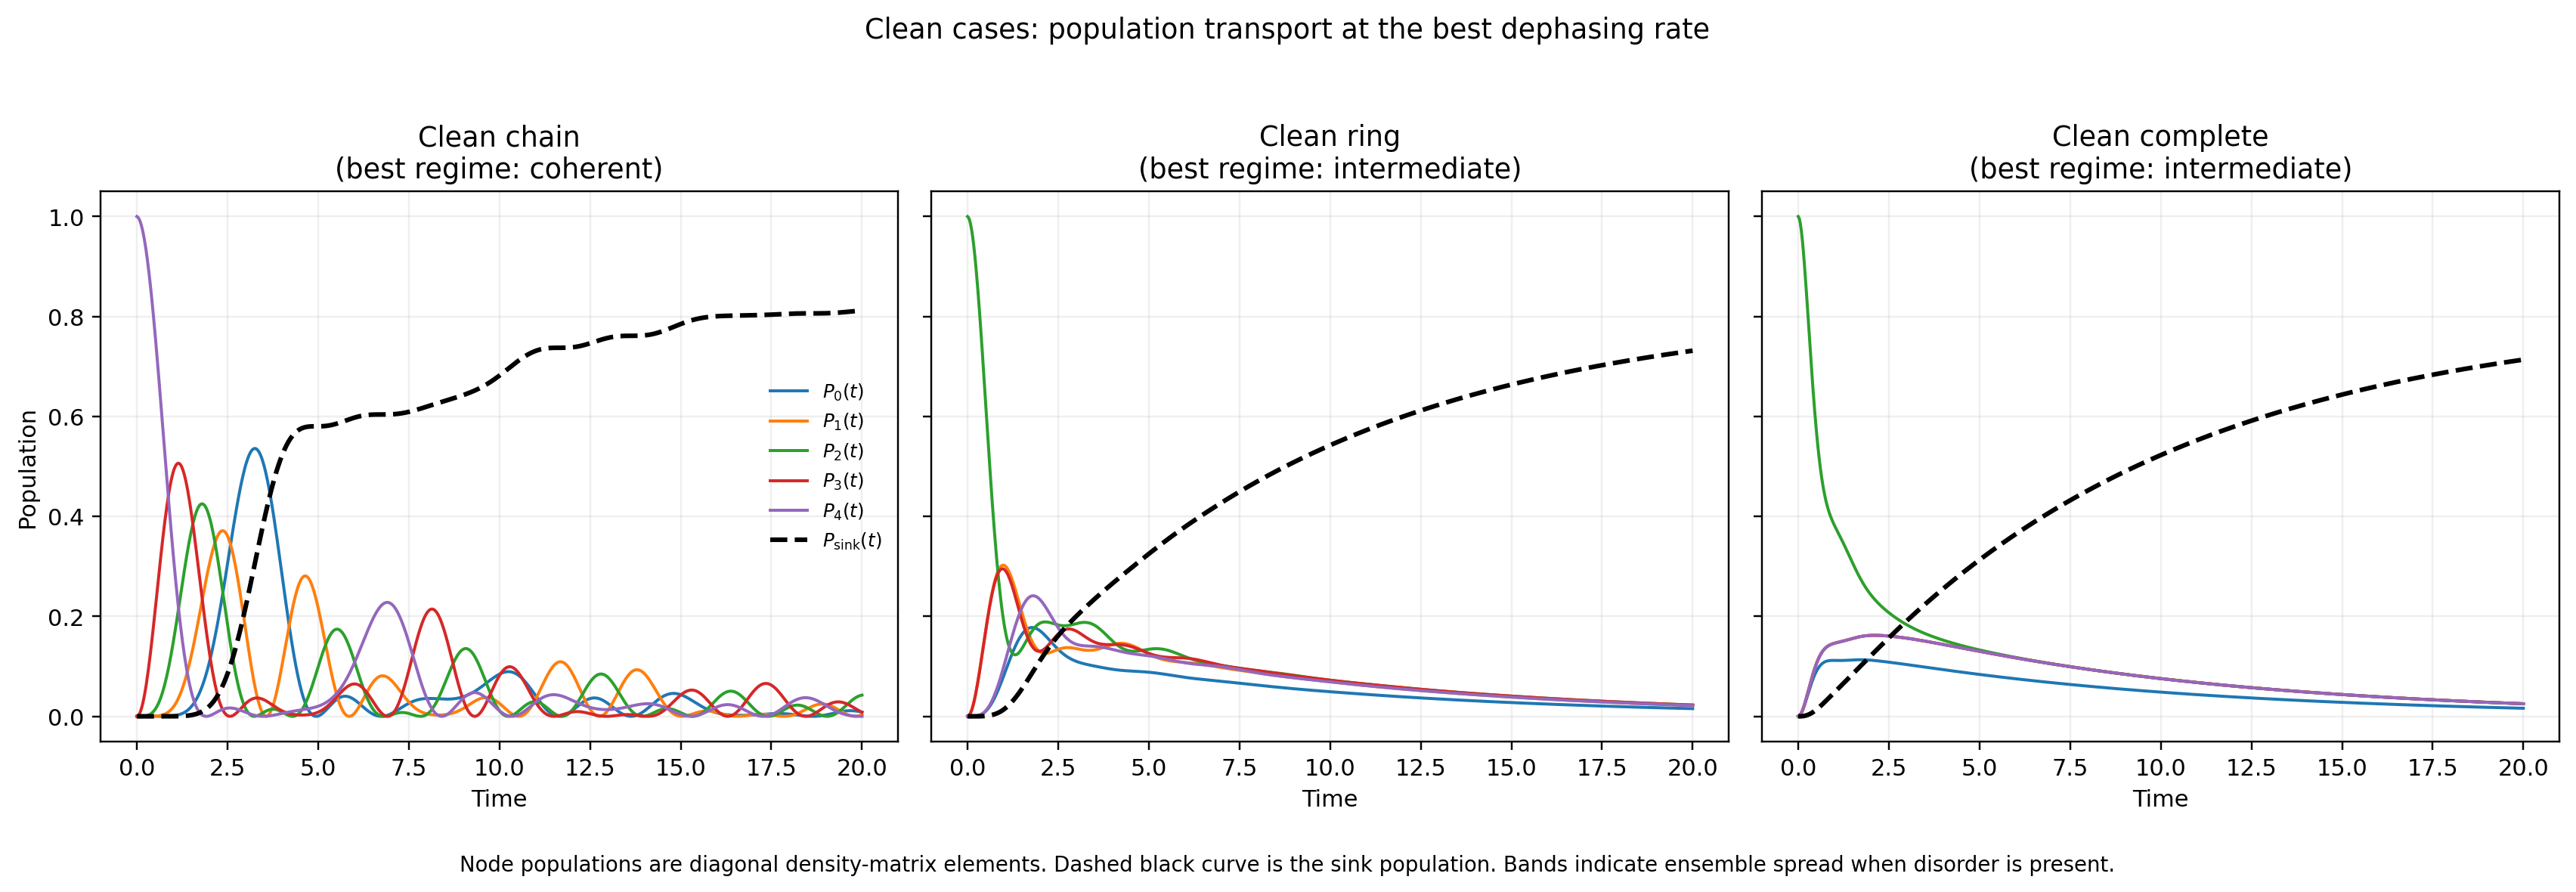
\includegraphics[width=\textwidth]{../../outputs/transport_networks/graph_collection/latest/figures/clean_population_dynamics.png}
  \caption{Population dynamics for the clean family at the dephasing rate that maximizes sink efficiency in each case. Each colored curve is a node population $P_i(t)=\rho_{ii}(t)$ and the dashed black curve is the sink population $P_s(t)=\rho_{ss}(t)$.}
\end{figure}

\begin{figure}[t]
  \centering
  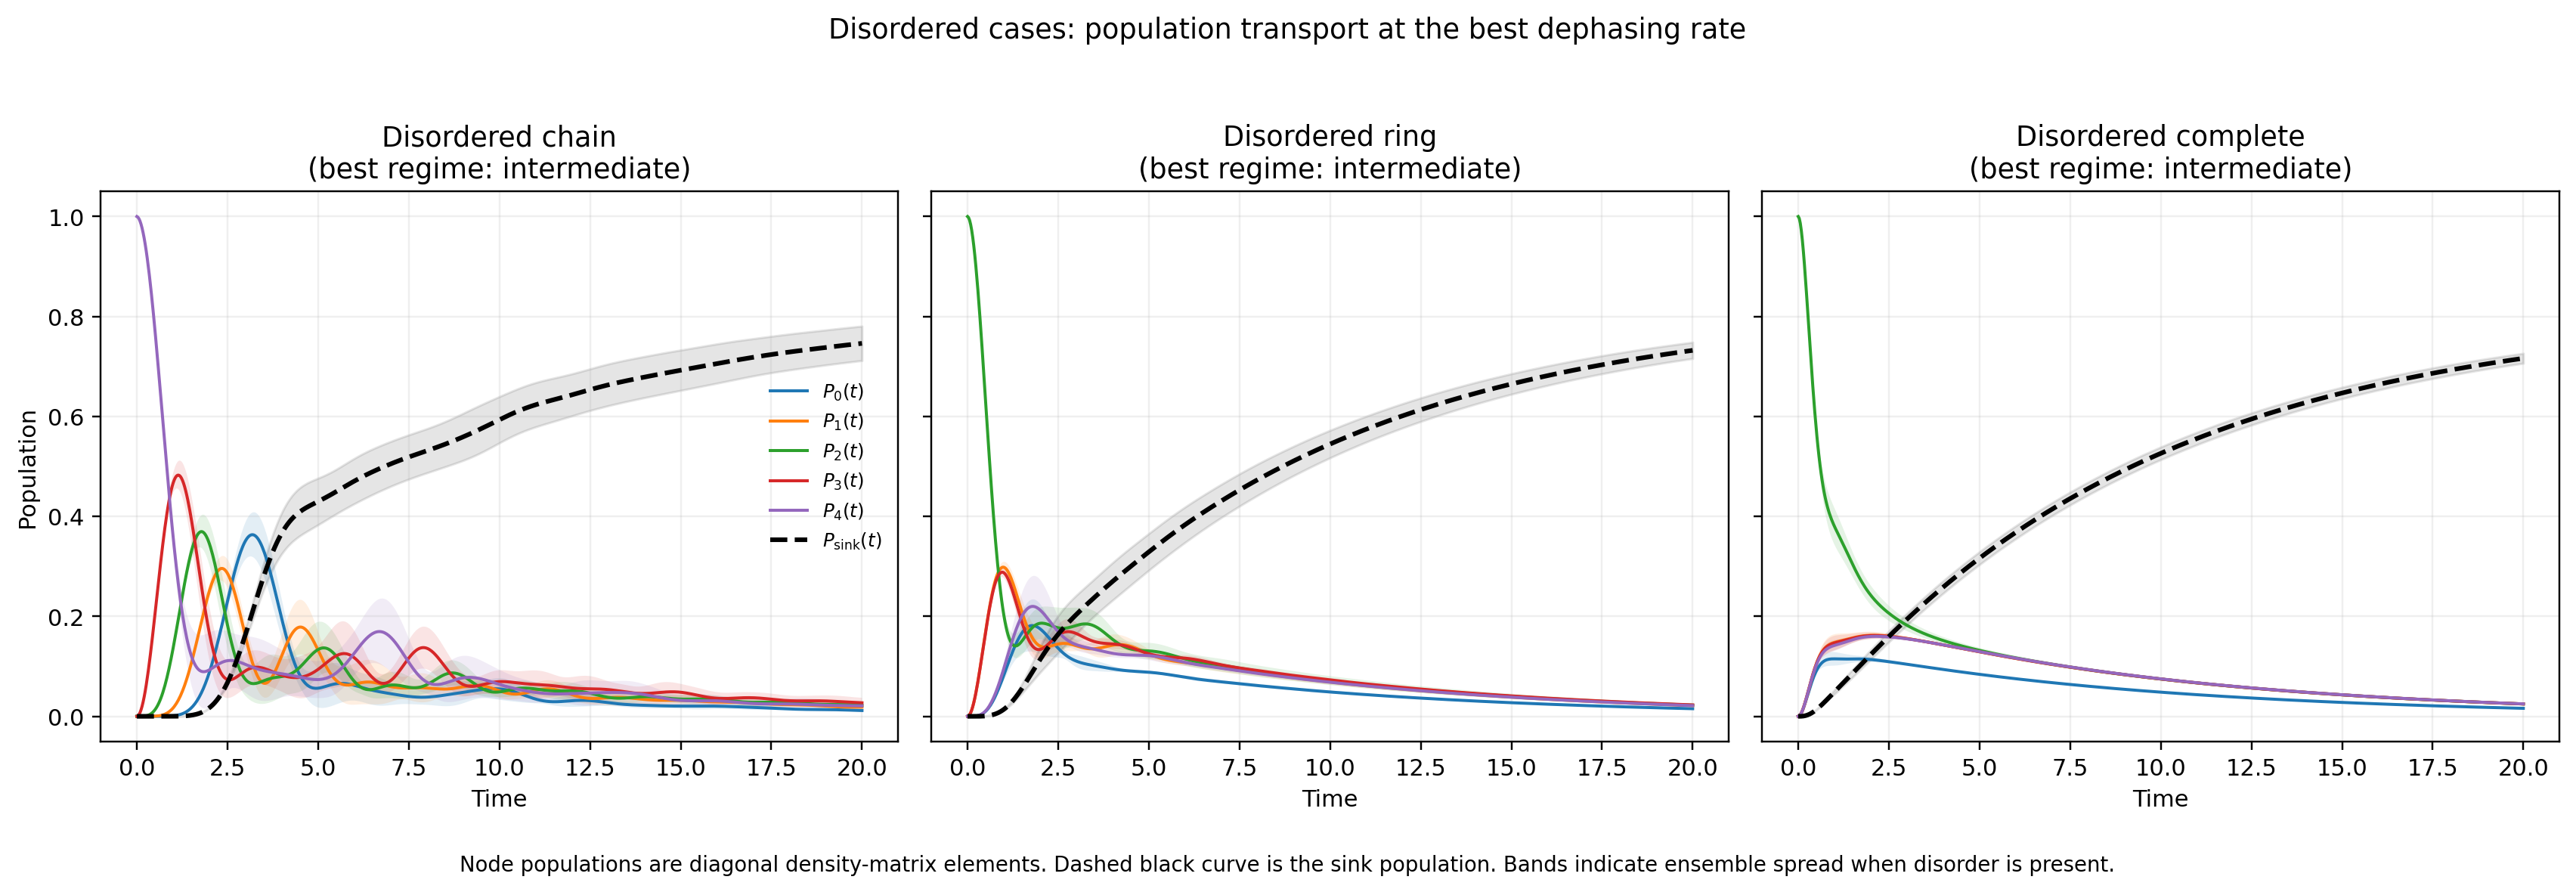
\includegraphics[width=\textwidth]{../../outputs/transport_networks/graph_collection/latest/figures/disordered_population_dynamics.png}
  \caption{Population dynamics for the disordered family at the best dephasing rate. The shaded bands are ensemble spreads across disorder realizations. They show how much the site-resolved transport pattern fluctuates when the on-site energies are randomized.}
\end{figure}

These plots answer a question that the sink-efficiency curves alone cannot
answer: \emph{how} does the excitation arrive? The sink curve can tell us that a
case is successful, but only the node-population curves show whether the
transfer is direct, oscillatory, bottlenecked, or broadly redistributed before
capture.

\section{Case-by-case comments}

\subsection{Clean chain}
This case uses a chain topology with 5 sites, initial site 4, trap site 0, coherent coupling $J=1.00$, sink rate $\kappa=0.65$, and loss rate $\Gamma=0.02$. The disorder strength is $W=0.00$ and the ensemble contains 1 realization(s).
The best regime is coherent, with $\eta_{\mathrm{best}}=0.812$, uncertainty $\sigma_\eta=0.000$, and optimal dephasing rate $\gamma_\phi^{\mathrm{best}}=0.000$. The mean coherence at the optimum is $C_{\ell_1}=0.734$.
The conditional final-state diagnostics at the optimum are purity $\gamma=1.000$, von Neumann entropy $S=0.000$, Shannon population entropy $H_\mathrm{pop}=0.955$, participation ratio $PR=1.993$, and inverse participation ratio $IPR=0.502$.
The numerical diagnostics at the optimum are $\max_t |\mathrm{Tr}\rho(t)-1|=6.22e-15$, $\max_t |\sum_i P_i(t)+P_s(t)+P_\ell(t)-1|=6.22e-15$, and minimum eigenvalue $\lambda_\mathrm{min}=-1.51e-15$. These values indicate that the reported populations are numerically trustworthy.
The coherent limit already gives the best transport, so additional dephasing mainly destroys phase relations that are helping the excitation reach the trap. The mean sink efficiency changes from 0.812 in the coherent limit to 0.812 at the optimum. At the optimum, the conditional network purity is 1.000, the conditional von Neumann entropy is 0.000, and the final participation ratio of the normalized node populations is 1.993. This is a deterministic clean-graph result, so the uncertainty is dominated by numerical diagnostics rather than ensemble spread.

\subsection{Clean ring}
This case uses a ring topology with 5 sites, initial site 2, trap site 0, coherent coupling $J=1.00$, sink rate $\kappa=0.65$, and loss rate $\Gamma=0.02$. The disorder strength is $W=0.00$ and the ensemble contains 1 realization(s).
The best regime is intermediate, with $\eta_{\mathrm{best}}=0.732$, uncertainty $\sigma_\eta=0.000$, and optimal dephasing rate $\gamma_\phi^{\mathrm{best}}=0.800$. The mean coherence at the optimum is $C_{\ell_1}=0.287$.
The conditional final-state diagnostics at the optimum are purity $\gamma=0.210$, von Neumann entropy $S=1.583$, Shannon population entropy $H_\mathrm{pop}=1.600$, participation ratio $PR=4.916$, and inverse participation ratio $IPR=0.203$.
The numerical diagnostics at the optimum are $\max_t |\mathrm{Tr}\rho(t)-1|=1.55e-15$, $\max_t |\sum_i P_i(t)+P_s(t)+P_\ell(t)-1|=1.55e-15$, and minimum eigenvalue $\lambda_\mathrm{min}=0.00e+00$. These values indicate that the reported populations are numerically trustworthy.
An intermediate dephasing rate improves transport, which is the operational signature of environment-assisted transport in this case. The mean sink efficiency changes from 0.439 in the coherent limit to 0.732 at the optimum. At the optimum, the conditional network purity is 0.210, the conditional von Neumann entropy is 1.583, and the final participation ratio of the normalized node populations is 4.916. This is a deterministic clean-graph result, so the uncertainty is dominated by numerical diagnostics rather than ensemble spread.

\subsection{Clean complete}
This case uses a complete topology with 5 sites, initial site 2, trap site 0, coherent coupling $J=1.00$, sink rate $\kappa=0.65$, and loss rate $\Gamma=0.02$. The disorder strength is $W=0.00$ and the ensemble contains 1 realization(s).
The best regime is intermediate, with $\eta_{\mathrm{best}}=0.714$, uncertainty $\sigma_\eta=0.000$, and optimal dephasing rate $\gamma_\phi^{\mathrm{best}}=3.200$. The mean coherence at the optimum is $C_{\ell_1}=0.144$.
The conditional final-state diagnostics at the optimum are purity $\gamma=0.207$, von Neumann entropy $S=1.591$, Shannon population entropy $H_\mathrm{pop}=1.596$, participation ratio $PR=4.883$, and inverse participation ratio $IPR=0.205$.
The numerical diagnostics at the optimum are $\max_t |\mathrm{Tr}\rho(t)-1|=8.22e-15$, $\max_t |\sum_i P_i(t)+P_s(t)+P_\ell(t)-1|=8.22e-15$, and minimum eigenvalue $\lambda_\mathrm{min}=0.00e+00$. These values indicate that the reported populations are numerically trustworthy.
An intermediate dephasing rate improves transport, which is the operational signature of environment-assisted transport in this case. The mean sink efficiency changes from 0.213 in the coherent limit to 0.714 at the optimum. At the optimum, the conditional network purity is 0.207, the conditional von Neumann entropy is 1.591, and the final participation ratio of the normalized node populations is 4.883. This is a deterministic clean-graph result, so the uncertainty is dominated by numerical diagnostics rather than ensemble spread.

\subsection{Disordered chain}
This case uses a chain topology with 5 sites, initial site 4, trap site 0, coherent coupling $J=1.00$, sink rate $\kappa=0.65$, and loss rate $\Gamma=0.02$. The disorder strength is $W=0.70$ and the ensemble contains 32 realization(s).
The best regime is intermediate, with $\eta_{\mathrm{best}}=0.746$, uncertainty $\sigma_\eta=0.034$, and optimal dephasing rate $\gamma_\phi^{\mathrm{best}}=0.100$. The mean coherence at the optimum is $C_{\ell_1}=0.700$.
The conditional final-state diagnostics at the optimum are purity $\gamma=0.306$, von Neumann entropy $S=1.372$, Shannon population entropy $H_\mathrm{pop}=1.558$, participation ratio $PR=4.546$, and inverse participation ratio $IPR=0.220$.
The numerical diagnostics at the optimum are $\max_t |\mathrm{Tr}\rho(t)-1|=9.21e-15$, $\max_t |\sum_i P_i(t)+P_s(t)+P_\ell(t)-1|=9.21e-15$, and minimum eigenvalue $\lambda_\mathrm{min}=0.00e+00$. These values indicate that the reported populations are numerically trustworthy.
An intermediate dephasing rate improves transport, which is the operational signature of environment-assisted transport in this case. The mean sink efficiency changes from 0.743 in the coherent limit to 0.746 at the optimum. At the optimum, the conditional network purity is 0.306, the conditional von Neumann entropy is 1.372, and the final participation ratio of the normalized node populations is 4.546. Static disorder is present, so the uncertainty bars quantify realization-to-realization variation across seeds rather than experimental measurement noise.

\subsection{Disordered ring}
This case uses a ring topology with 5 sites, initial site 2, trap site 0, coherent coupling $J=1.00$, sink rate $\kappa=0.65$, and loss rate $\Gamma=0.02$. The disorder strength is $W=0.70$ and the ensemble contains 32 realization(s).
The best regime is intermediate, with $\eta_{\mathrm{best}}=0.732$, uncertainty $\sigma_\eta=0.016$, and optimal dephasing rate $\gamma_\phi^{\mathrm{best}}=0.800$. The mean coherence at the optimum is $C_{\ell_1}=0.285$.
The conditional final-state diagnostics at the optimum are purity $\gamma=0.211$, von Neumann entropy $S=1.581$, Shannon population entropy $H_\mathrm{pop}=1.599$, participation ratio $PR=4.903$, and inverse participation ratio $IPR=0.204$.
The numerical diagnostics at the optimum are $\max_t |\mathrm{Tr}\rho(t)-1|=9.99e-15$, $\max_t |\sum_i P_i(t)+P_s(t)+P_\ell(t)-1|=9.99e-15$, and minimum eigenvalue $\lambda_\mathrm{min}=0.00e+00$. These values indicate that the reported populations are numerically trustworthy.
An intermediate dephasing rate improves transport, which is the operational signature of environment-assisted transport in this case. The mean sink efficiency changes from 0.623 in the coherent limit to 0.732 at the optimum. At the optimum, the conditional network purity is 0.211, the conditional von Neumann entropy is 1.581, and the final participation ratio of the normalized node populations is 4.903. Static disorder is present, so the uncertainty bars quantify realization-to-realization variation across seeds rather than experimental measurement noise.

\subsection{Disordered complete}
This case uses a complete topology with 5 sites, initial site 2, trap site 0, coherent coupling $J=1.00$, sink rate $\kappa=0.65$, and loss rate $\Gamma=0.02$. The disorder strength is $W=0.70$ and the ensemble contains 32 realization(s).
The best regime is intermediate, with $\eta_{\mathrm{best}}=0.716$, uncertainty $\sigma_\eta=0.010$, and optimal dephasing rate $\gamma_\phi^{\mathrm{best}}=3.200$. The mean coherence at the optimum is $C_{\ell_1}=0.143$.
The conditional final-state diagnostics at the optimum are purity $\gamma=0.206$, von Neumann entropy $S=1.592$, Shannon population entropy $H_\mathrm{pop}=1.597$, participation ratio $PR=4.886$, and inverse participation ratio $IPR=0.205$.
The numerical diagnostics at the optimum are $\max_t |\mathrm{Tr}\rho(t)-1|=9.77e-15$, $\max_t |\sum_i P_i(t)+P_s(t)+P_\ell(t)-1|=9.77e-15$, and minimum eigenvalue $\lambda_\mathrm{min}=0.00e+00$. These values indicate that the reported populations are numerically trustworthy.
An intermediate dephasing rate improves transport, which is the operational signature of environment-assisted transport in this case. The mean sink efficiency changes from 0.375 in the coherent limit to 0.716 at the optimum. At the optimum, the conditional network purity is 0.206, the conditional von Neumann entropy is 1.592, and the final participation ratio of the normalized node populations is 4.886. Static disorder is present, so the uncertainty bars quantify realization-to-realization variation across seeds rather than experimental measurement noise.


\section{Pairwise tables}

\begin{table}[t]
\centering
\caption{Pairwise differences in best sink efficiency for the clean cases. Entry $(i,j)$ is $\eta_{\mathrm{best},i}-\eta_{\mathrm{best},j}$.}
\begin{tabular}{lccc}
\toprule
Case & Clean chain & Clean ring & Clean complete \\
\midrule
Clean chain & +0.000 & +0.081 & +0.098 \\
Clean ring & -0.081 & +0.000 & +0.018 \\
Clean complete & -0.098 & -0.018 & +0.000 \\
\bottomrule
\end{tabular}
\end{table}

\begin{table}[t]
\centering
\caption{Pairwise differences in best sink efficiency for the disordered cases. Entry $(i,j)$ is $\eta_{\mathrm{best},i}-\eta_{\mathrm{best},j}$.}
\begin{tabular}{lccc}
\toprule
Case & Disordered chain & Disordered ring & Disordered complete \\
\midrule
Disordered chain & +0.000 & +0.014 & +0.030 \\
Disordered ring & -0.014 & +0.000 & +0.016 \\
Disordered complete & -0.030 & -0.016 & +0.000 \\
\bottomrule
\end{tabular}
\end{table}


\section{Targeted follow-up studies}

The next layer of the project is no longer a generic graph-family comparison. It is a set of targeted tests motivated by the first-pass atlas: a refined disorder scan for the chain, a denser size scan for the ring, a controlled ring study that separates parity from distance to the trap, and a sink-position sweep for all currently implemented topologies.

\begin{figure}[t]
\centering
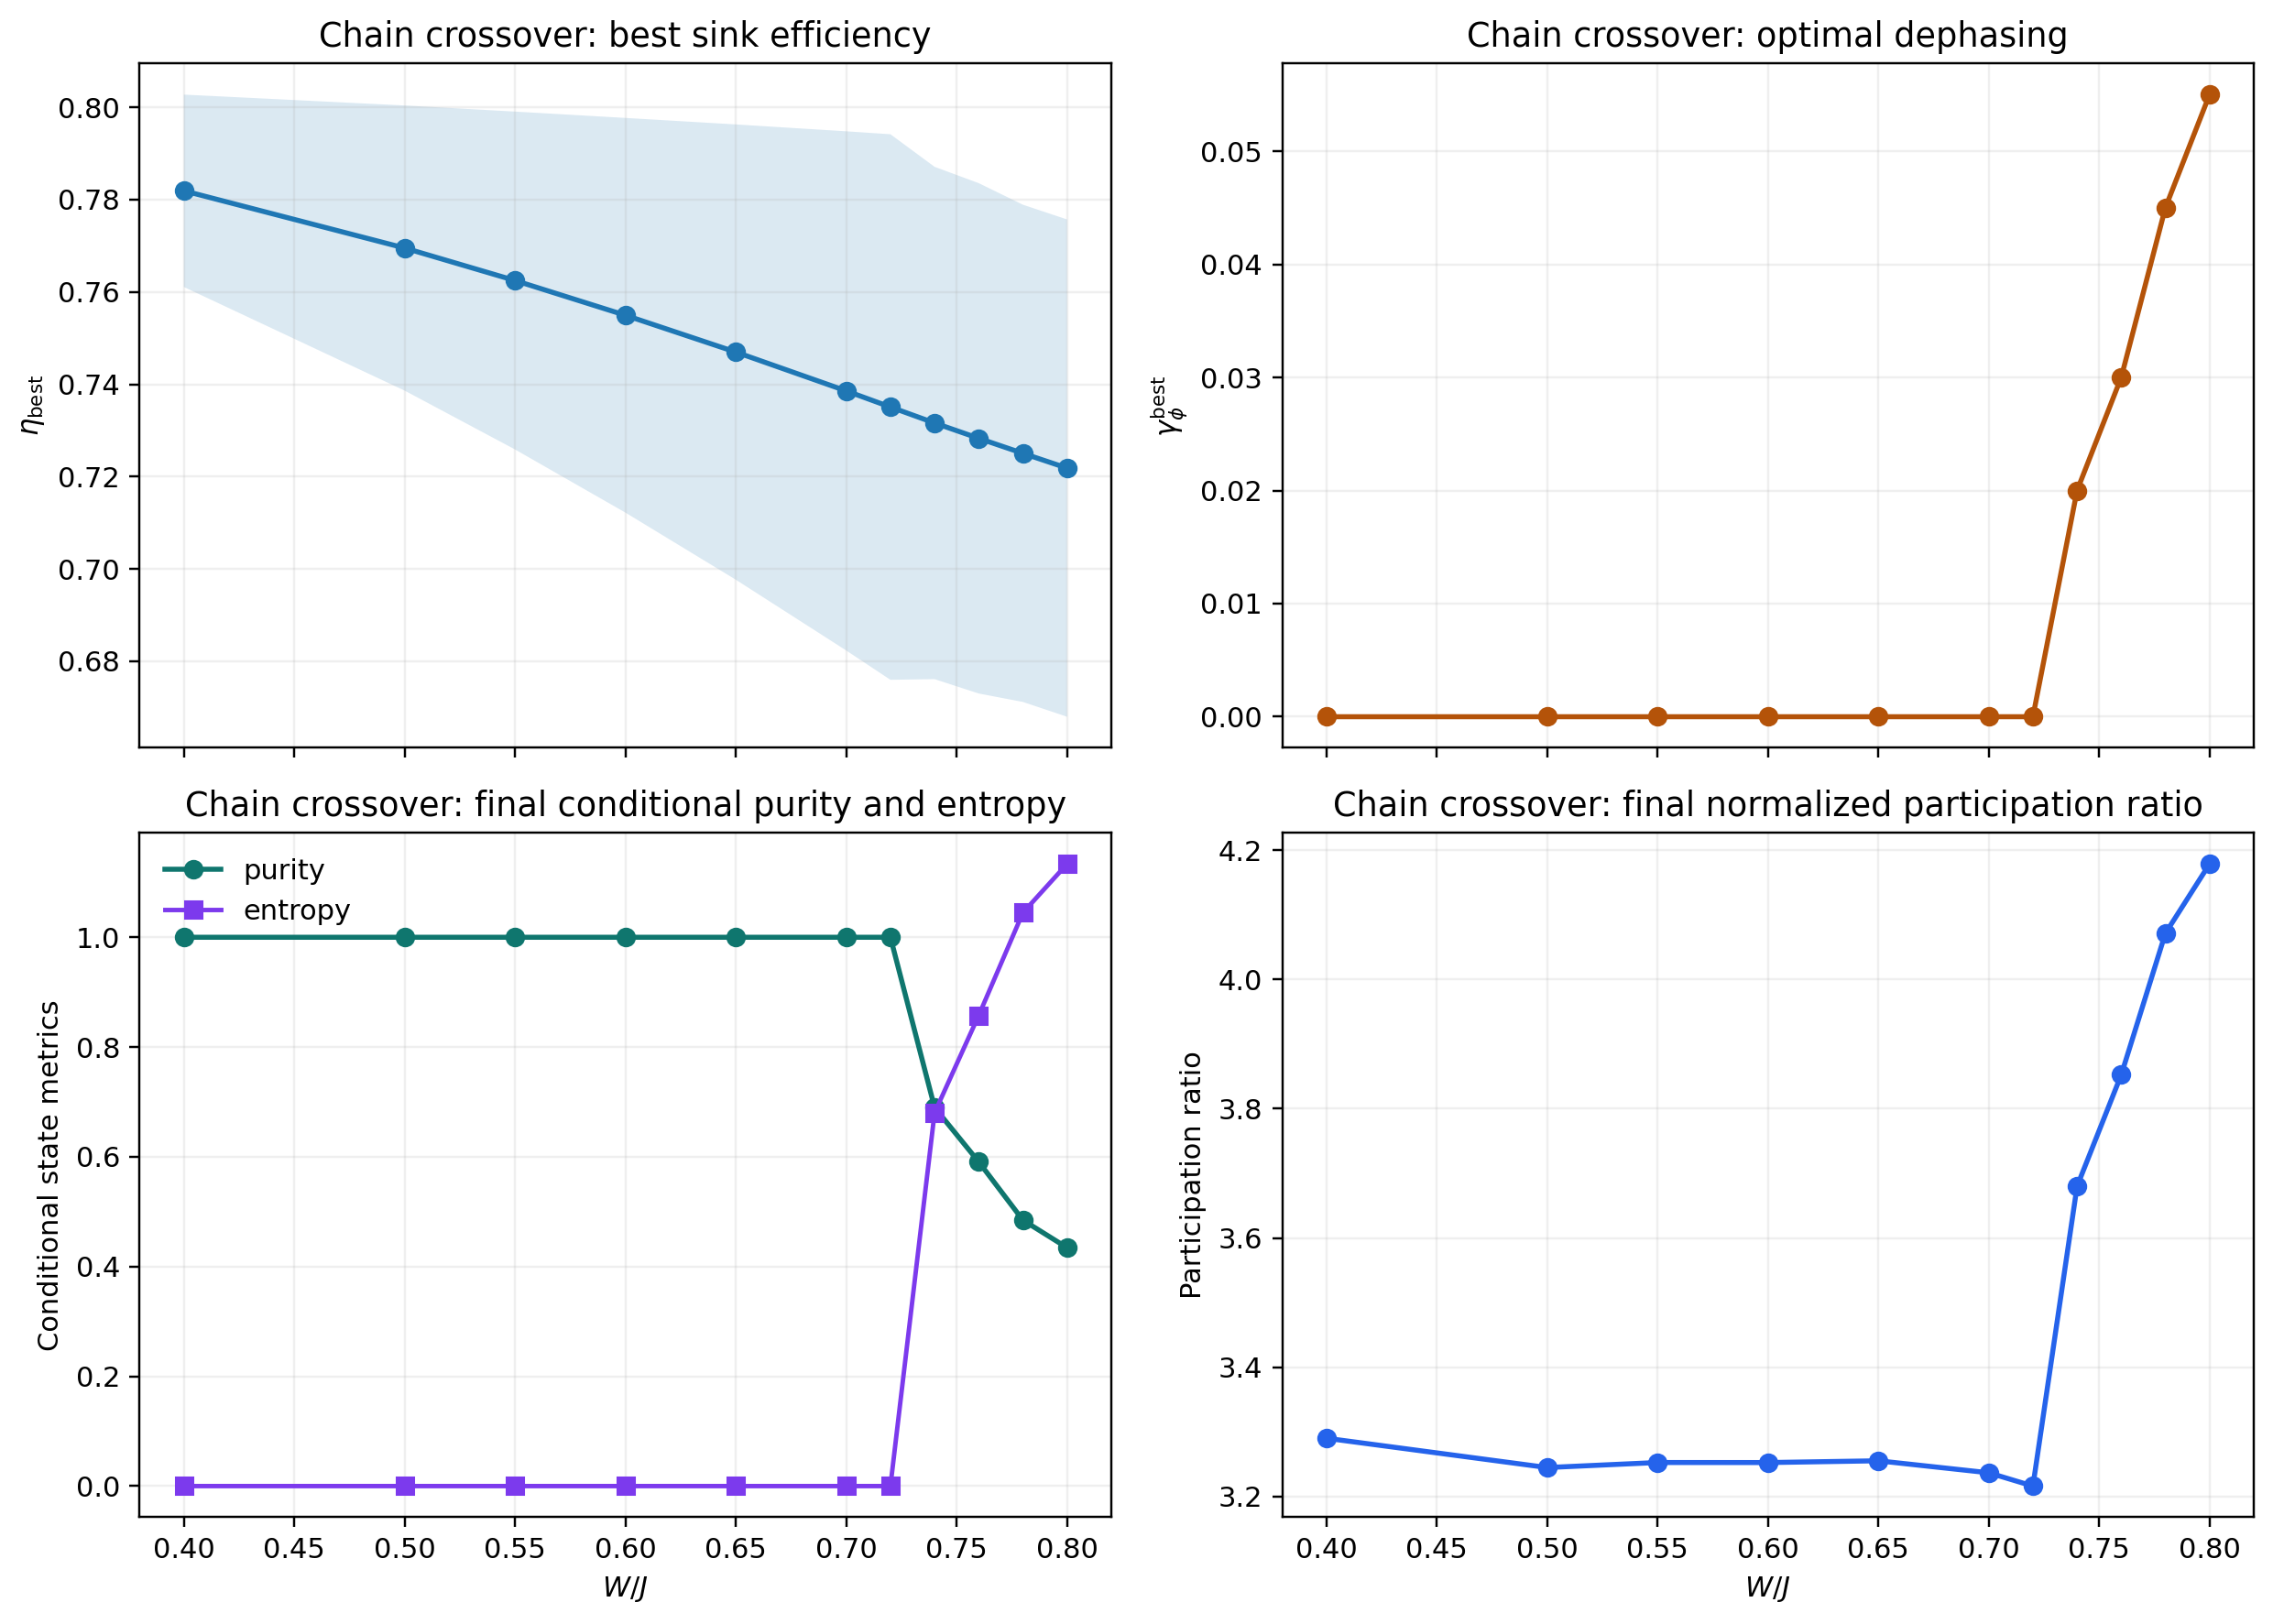
\includegraphics[width=0.86\textwidth]{../../outputs/transport_networks/targeted_studies/latest/figures/chain_crossover_refined.png}
\caption{Refined chain crossover study. Top-left: best sink efficiency versus $W/J$. Top-right: optimal dephasing versus $W/J$. Bottom panels: final conditional purity, entropy, and participation ratio at the transport optimum.}
\end{figure}

\begin{figure}[t]
\centering
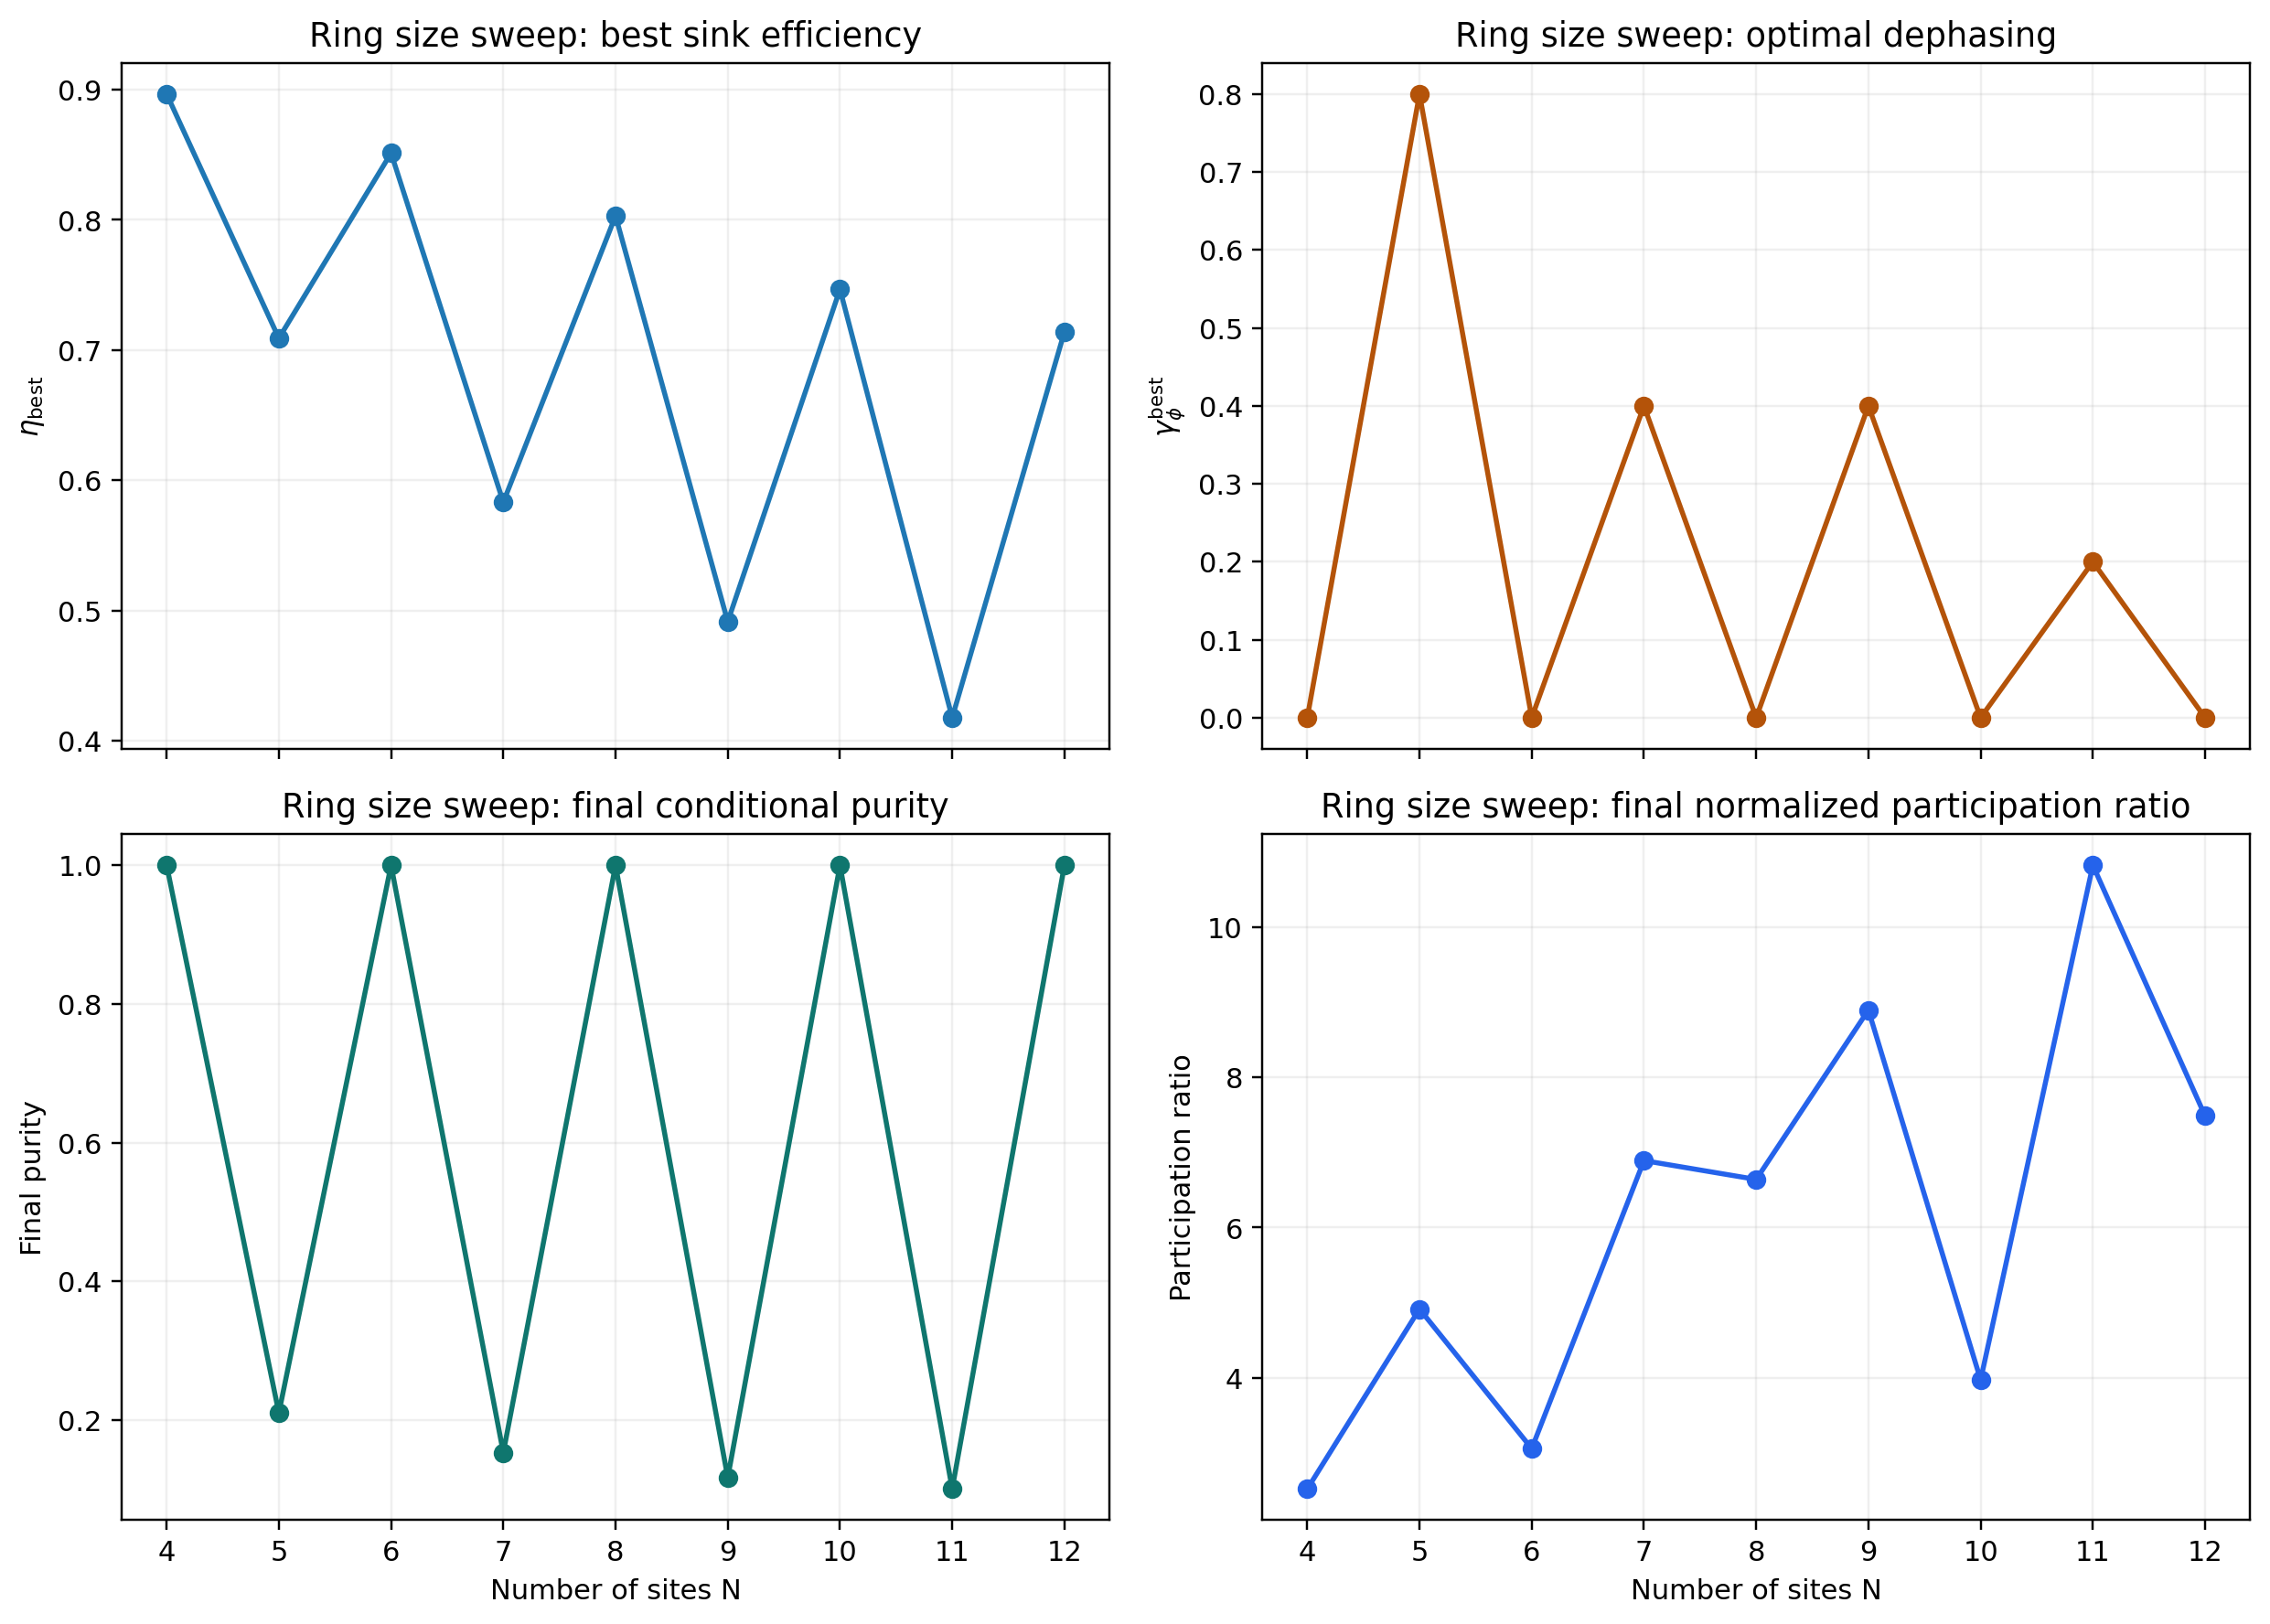
\includegraphics[width=0.86\textwidth]{../../outputs/transport_networks/targeted_studies/latest/figures/ring_size_refined.png}
\caption{Refined ring-size study. The goal is to test whether the original alternation between coherent-optimal and intermediate-optimal behavior is a real parity/symmetry effect.}
\end{figure}

\begin{figure}[t]
\centering
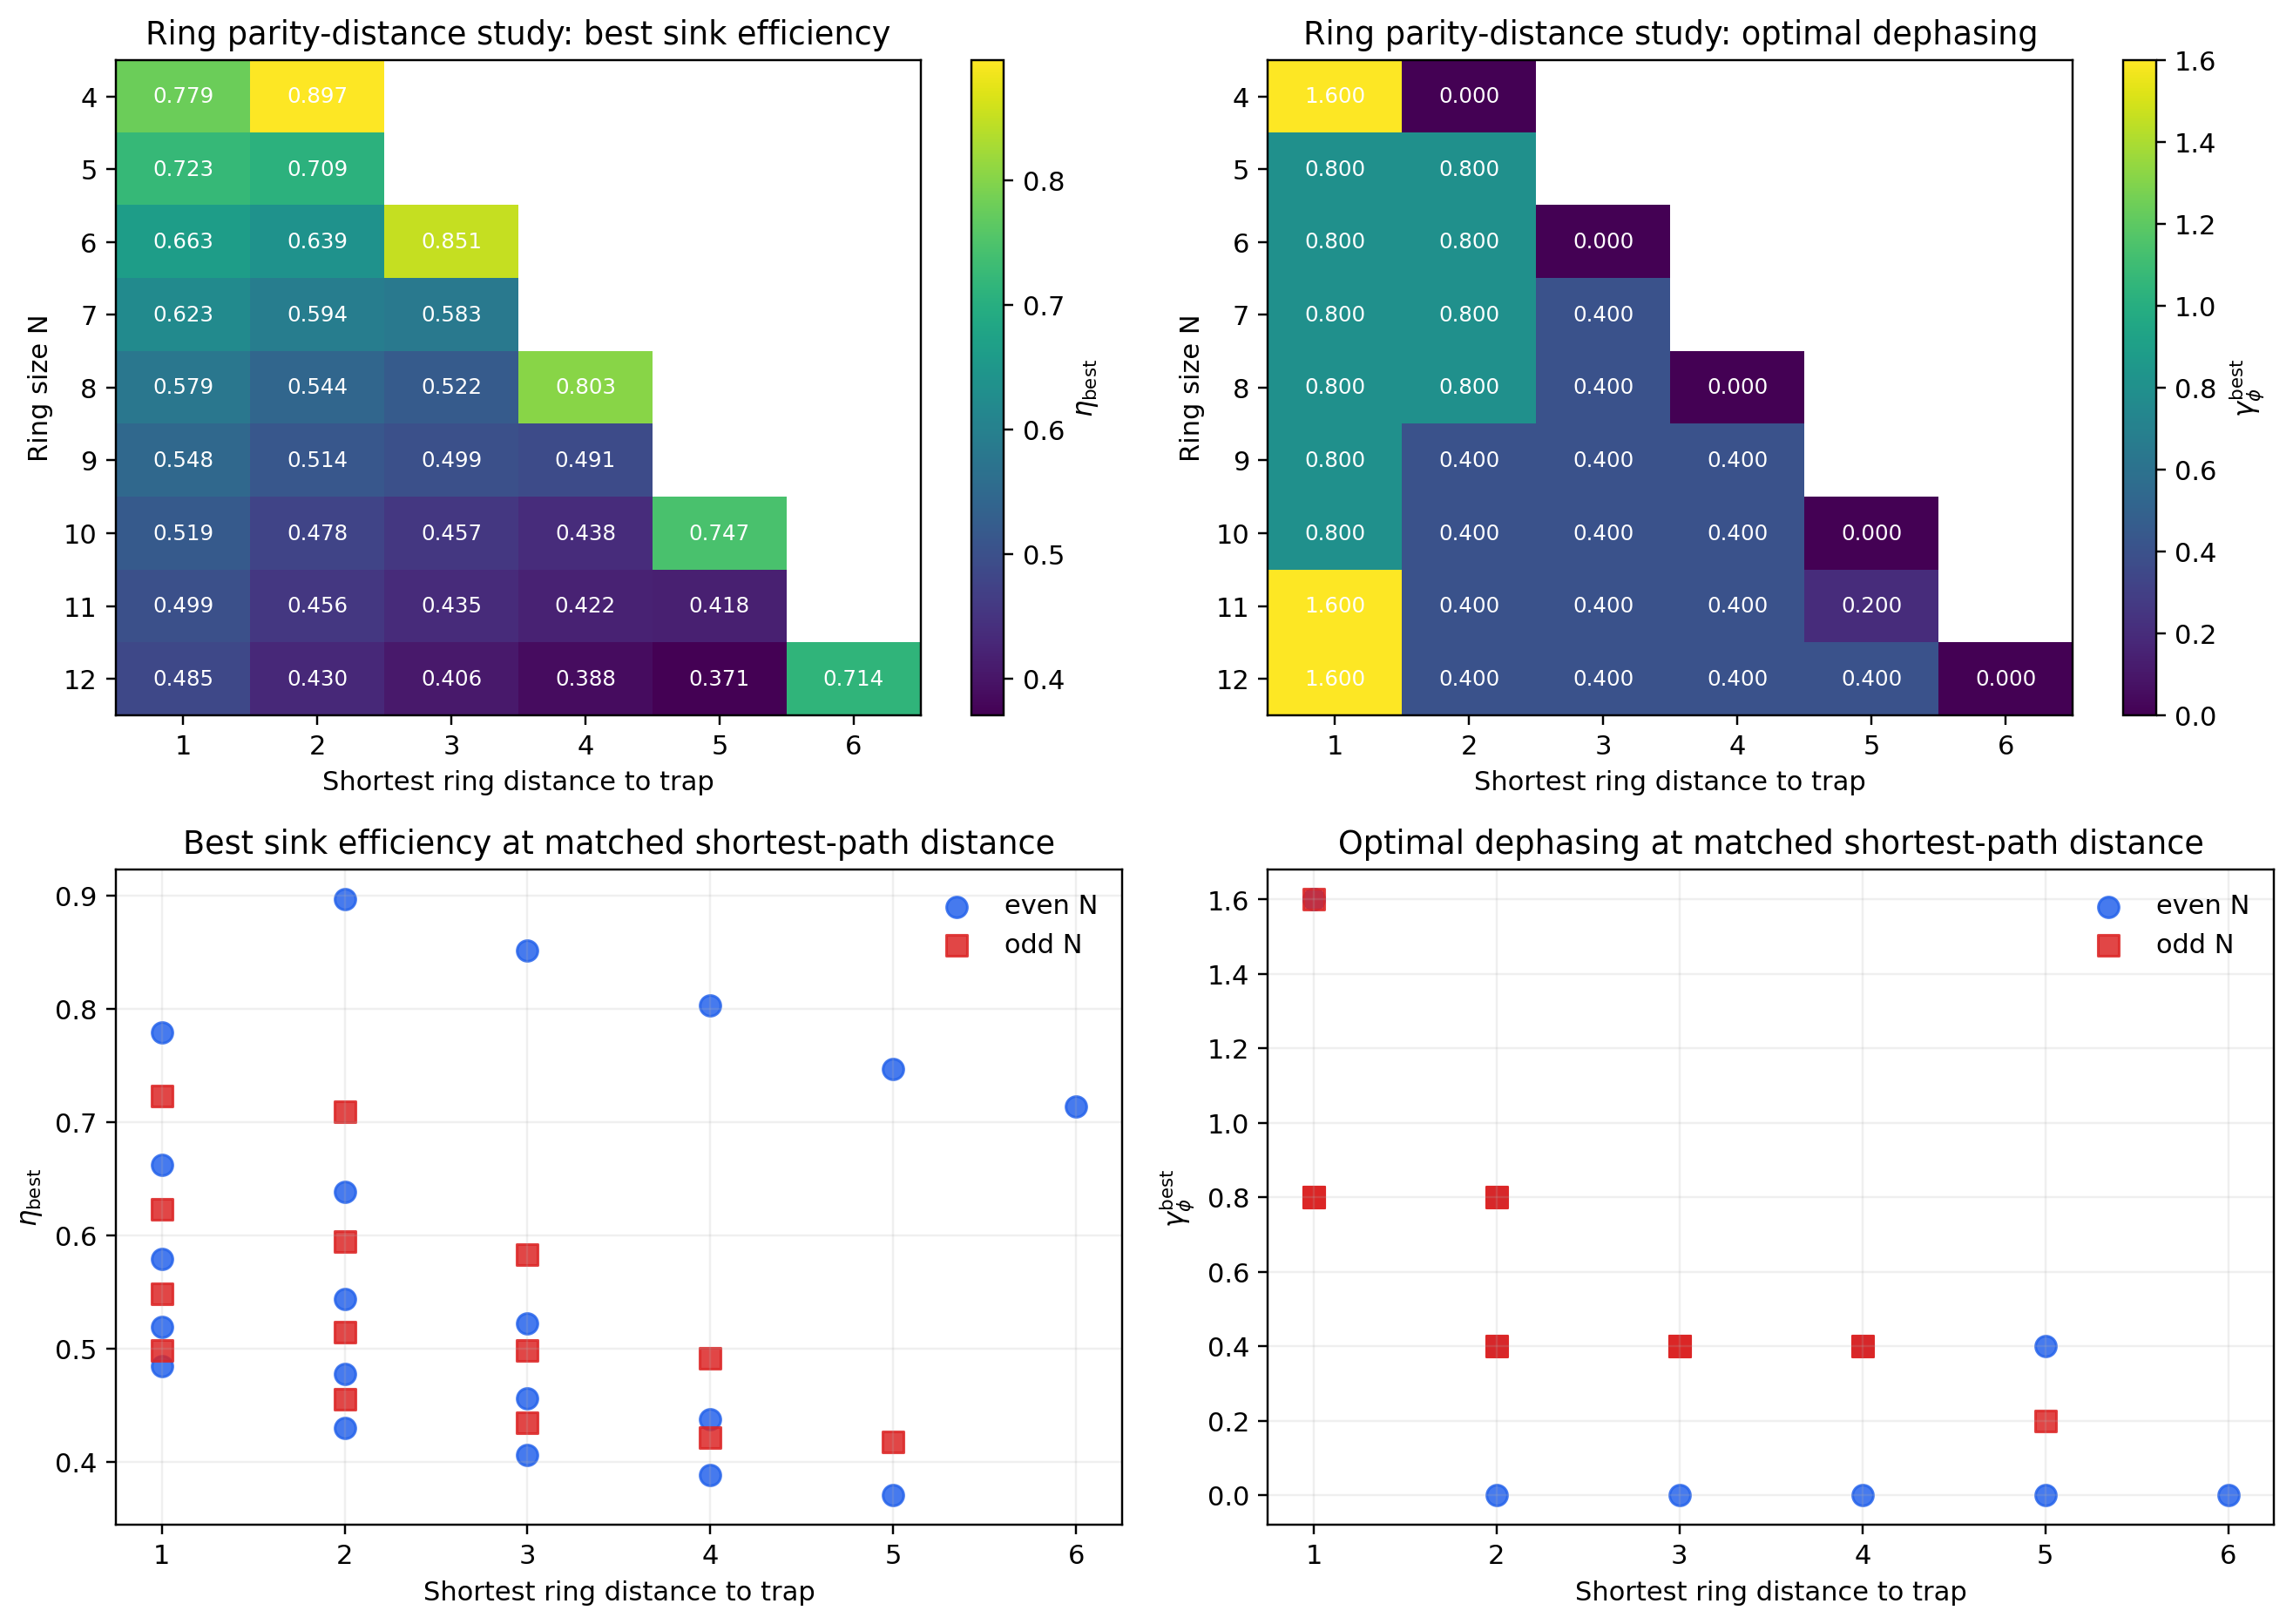
\includegraphics[width=0.86\textwidth]{../../outputs/transport_networks/targeted_studies/latest/figures/ring_parity_distance.png}
\caption{Controlled ring study that separates ring-size parity from shortest-path distance to the trap. Top panels: heat maps of best efficiency and optimal dephasing over $(N,d)$. Bottom panels: matched-distance comparisons between odd and even rings.}
\end{figure}

\begin{figure}[t]
\centering
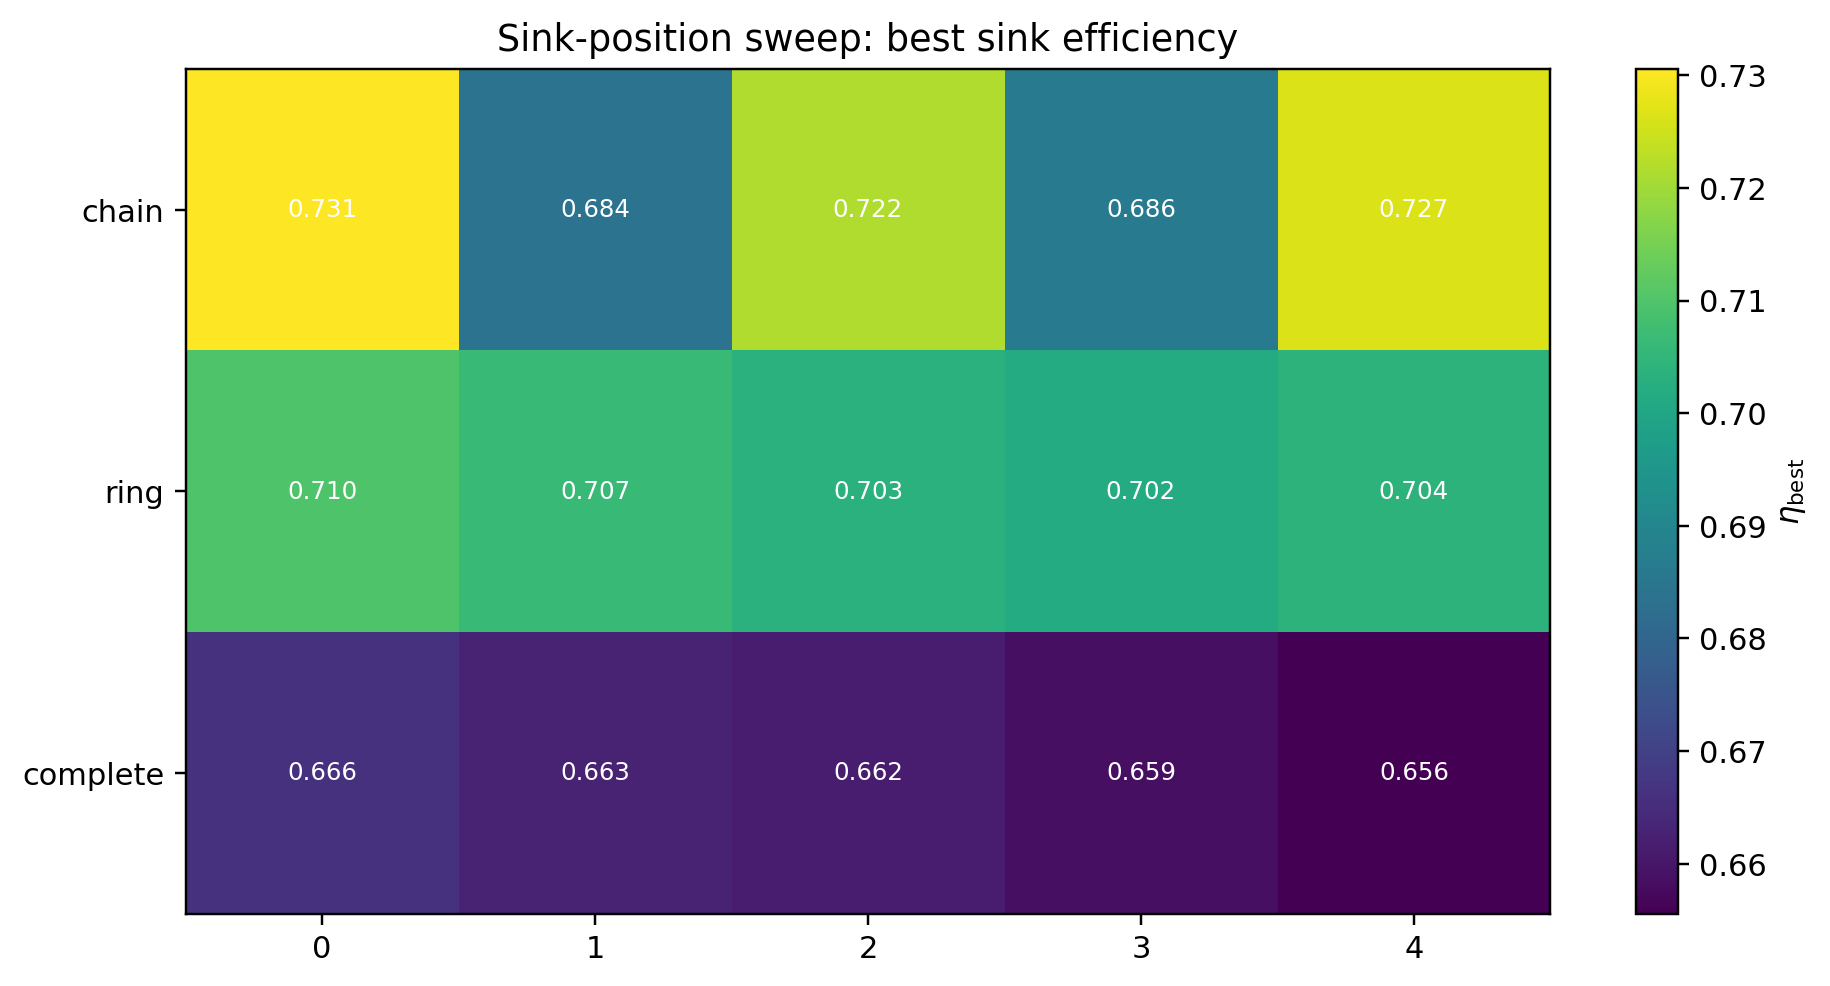
\includegraphics[width=0.48\textwidth]{../../outputs/transport_networks/targeted_studies/latest/figures/sink_position_eta_heatmap.png}
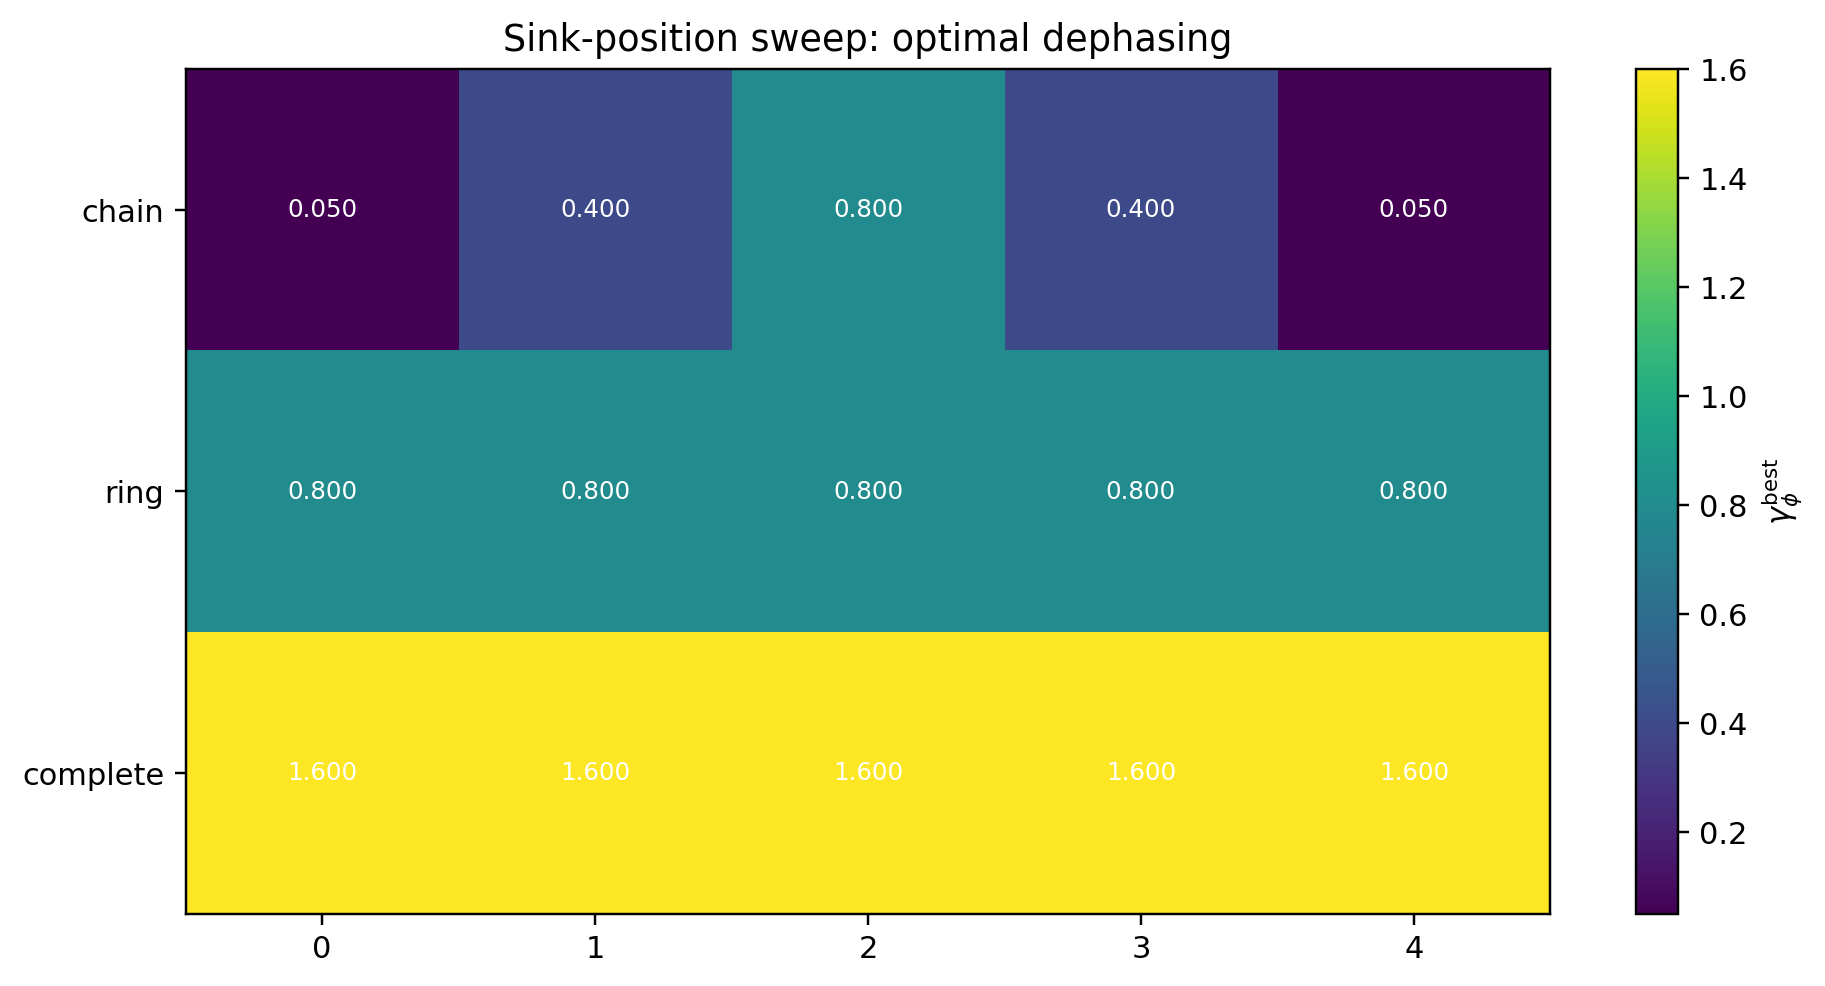
\includegraphics[width=0.48\textwidth]{../../outputs/transport_networks/targeted_studies/latest/figures/sink_position_gamma_heatmap.png}
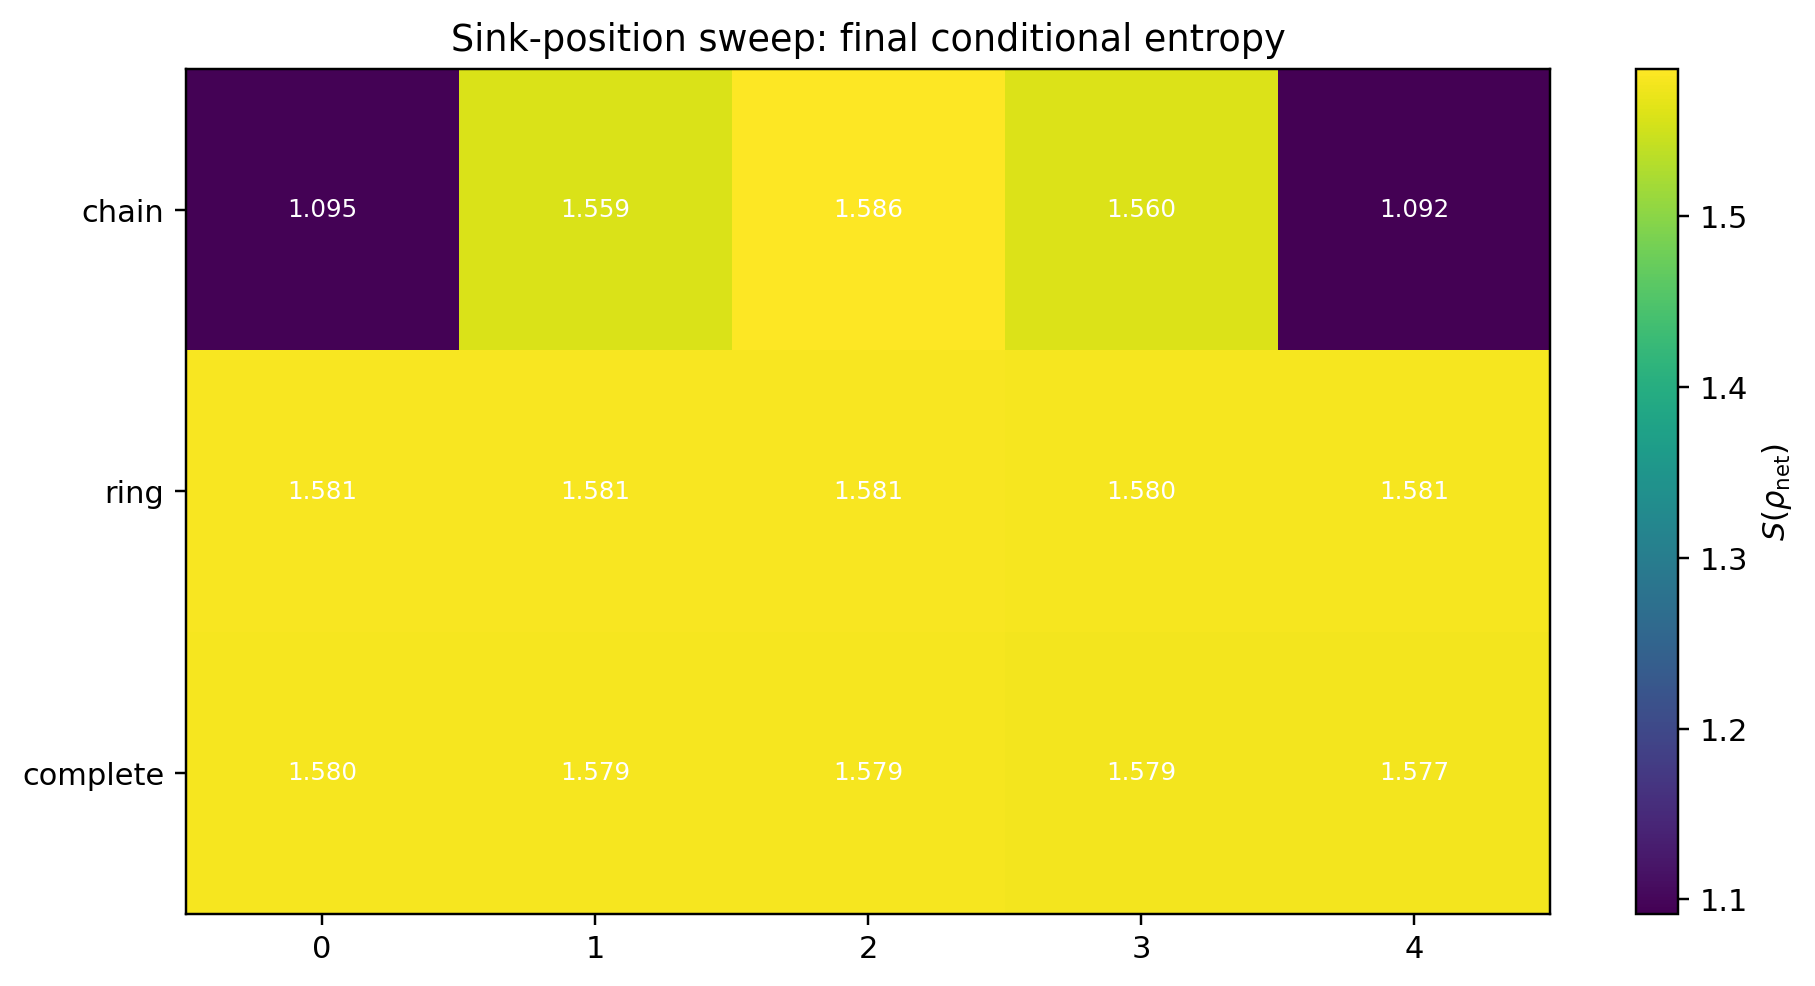
\includegraphics[width=0.48\textwidth]{../../outputs/transport_networks/targeted_studies/latest/figures/sink_position_entropy_heatmap.png}
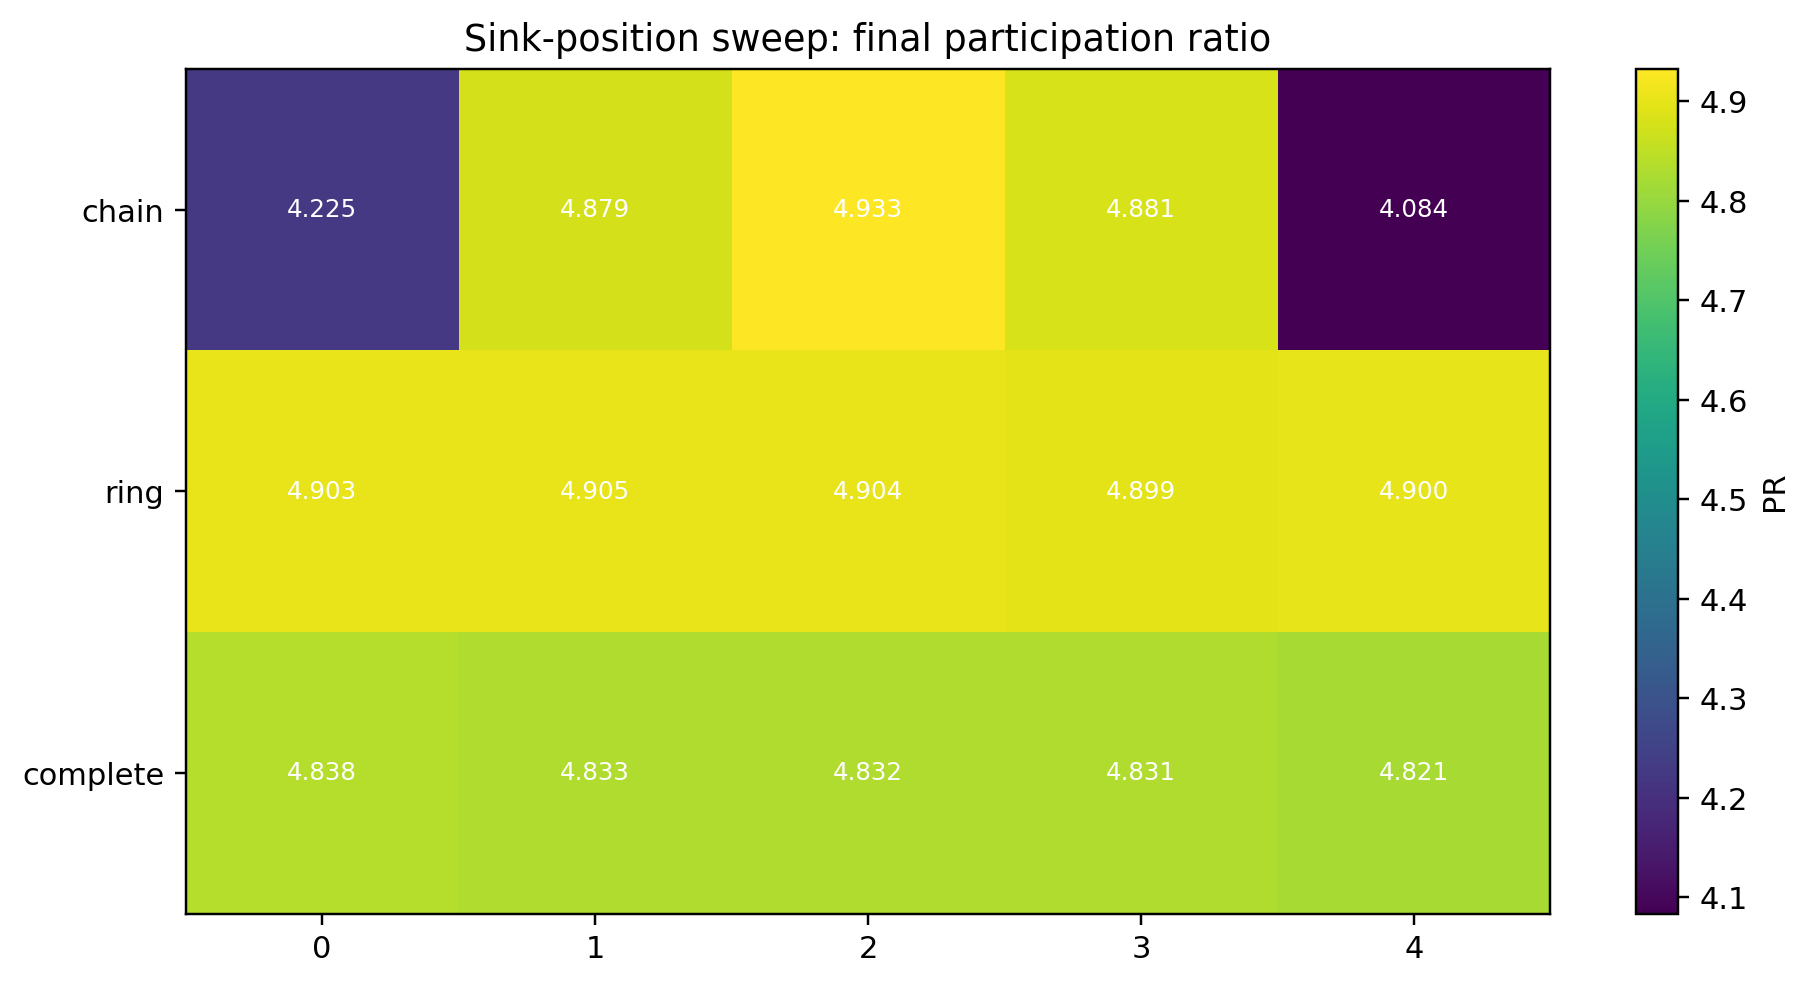
\includegraphics[width=0.48\textwidth]{../../outputs/transport_networks/targeted_studies/latest/figures/sink_position_participation_heatmap.png}
\caption{Sink-position sweep. Top-left: best transport efficiency. Top-right: optimal dephasing. Bottom-left: final conditional entropy. Bottom-right: final participation ratio. The sweep uses a 32-seed disorder ensemble.}
\end{figure}

\begin{figure}[t]
\centering
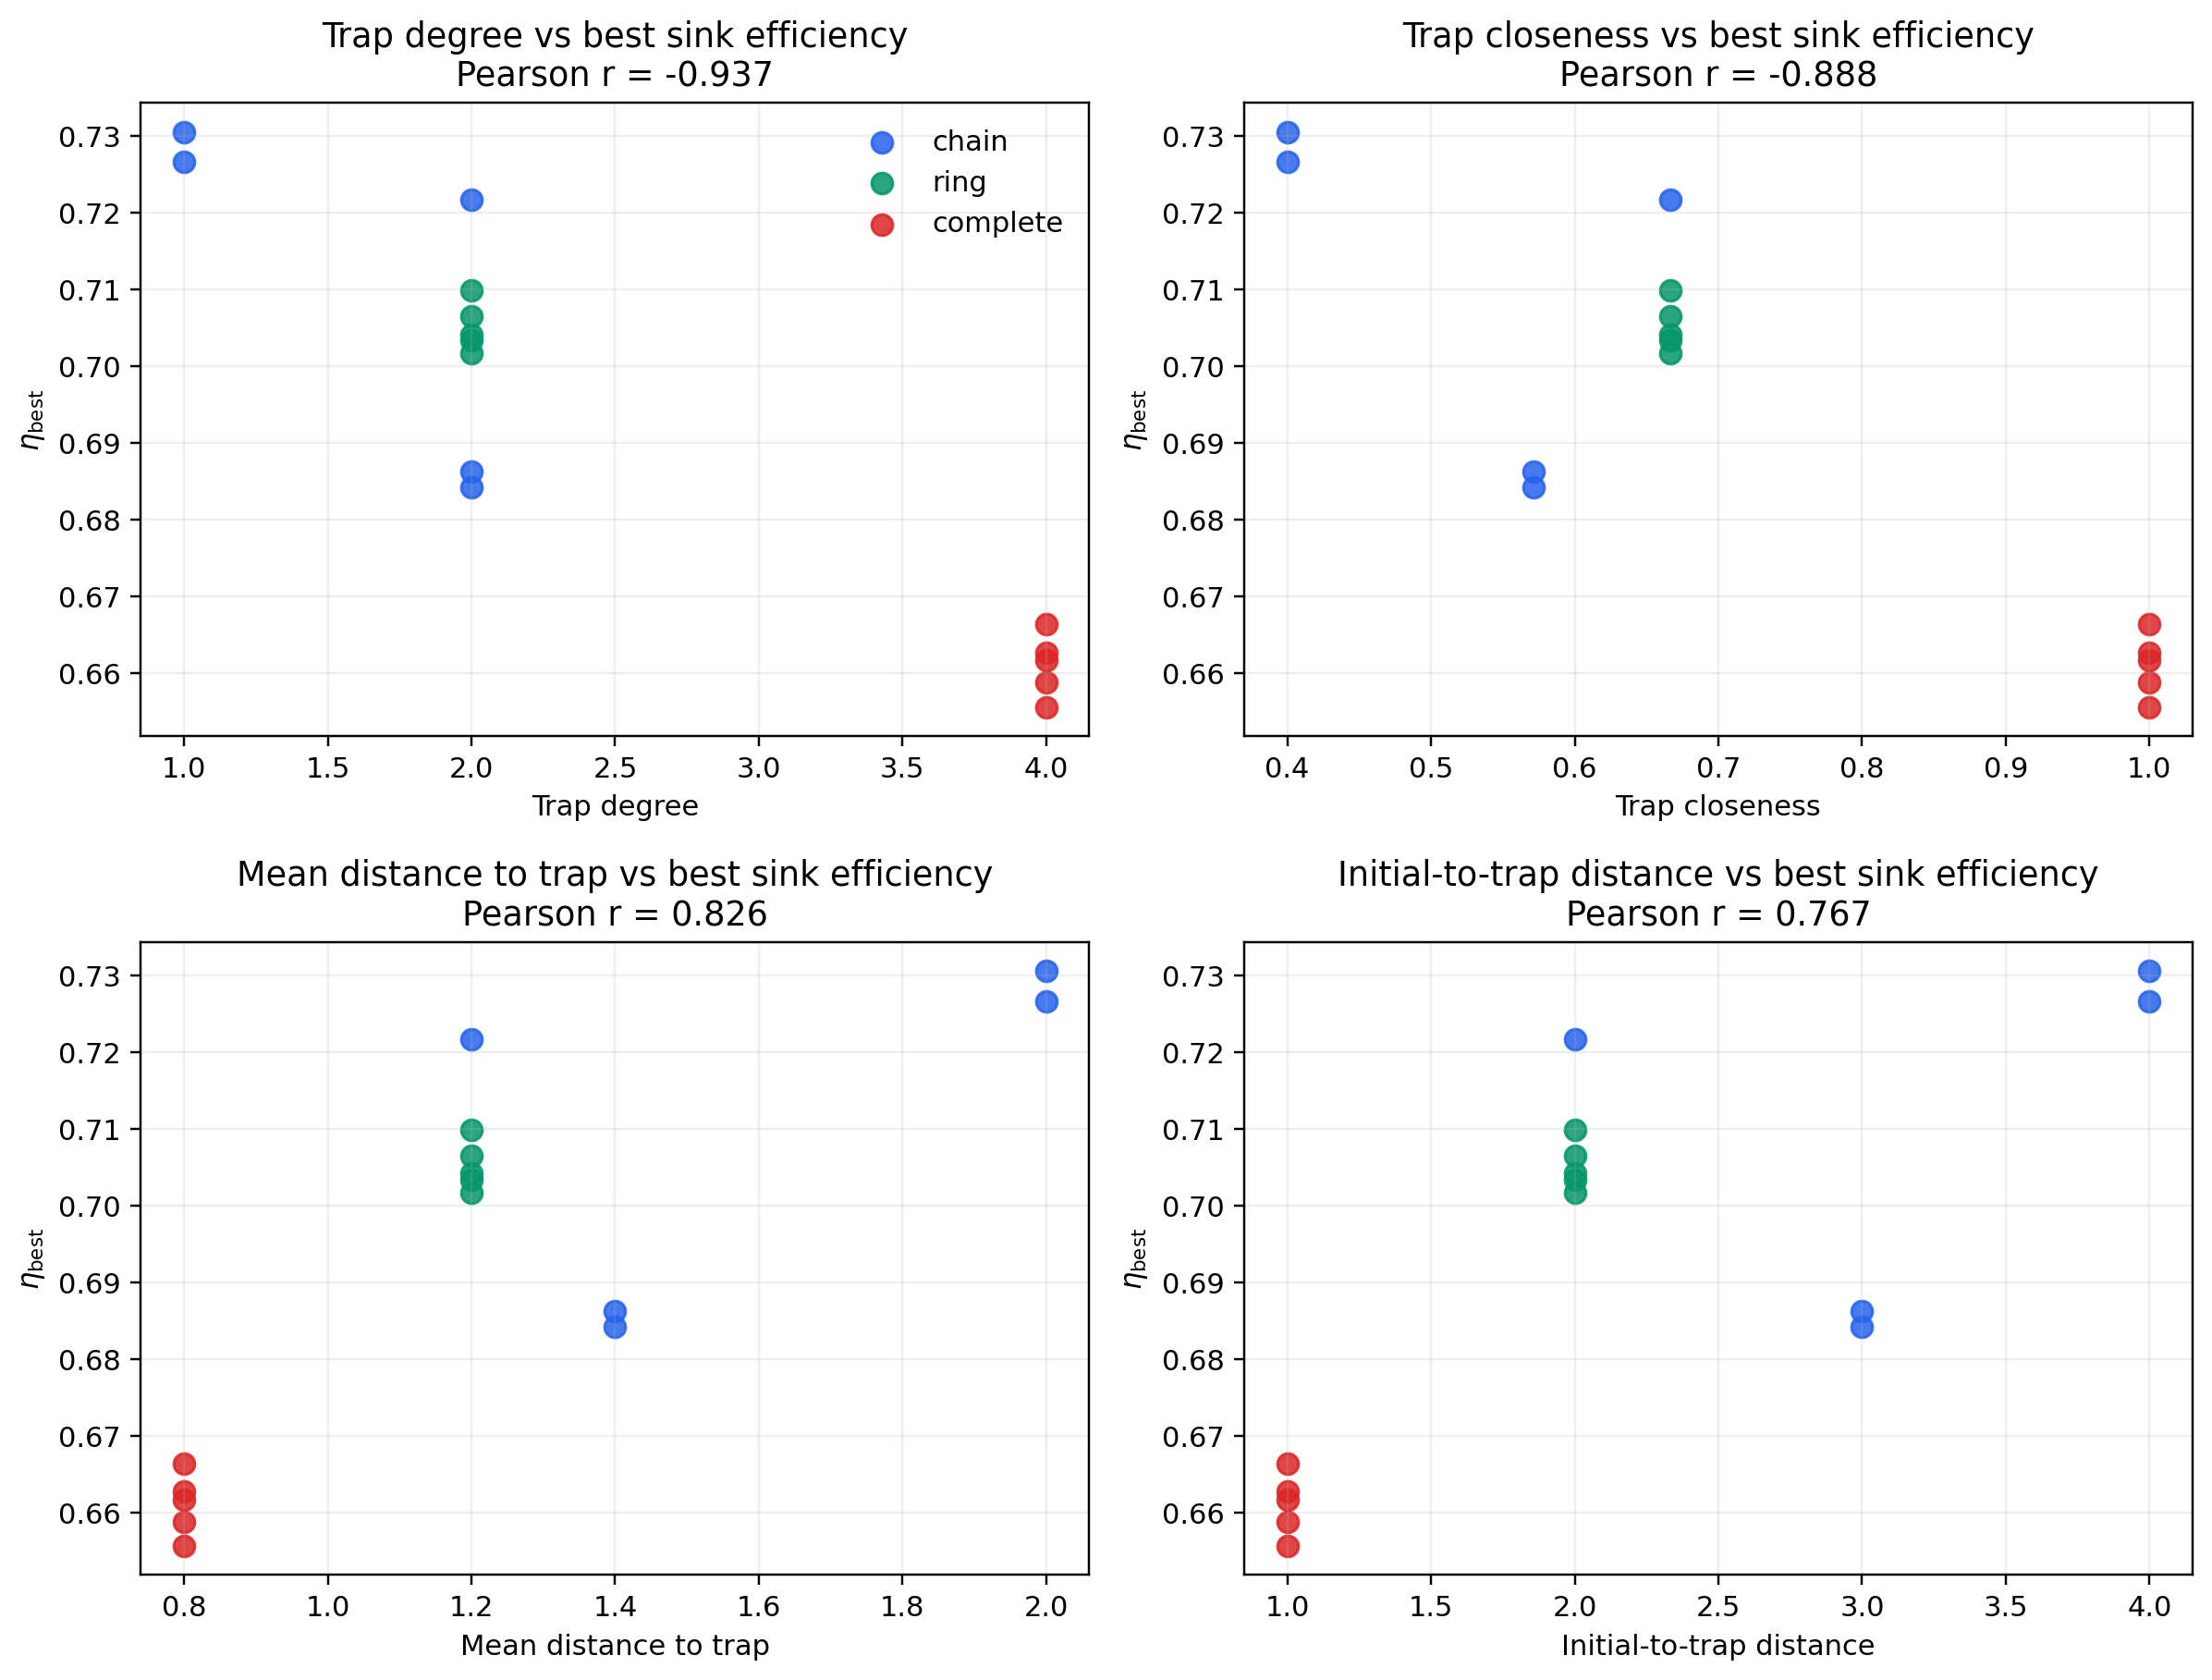
\includegraphics[width=0.86\textwidth]{../../outputs/transport_networks/targeted_studies/latest/figures/sink_position_metric_correlations.png}
\caption{Correlations between graph metrics of the trap node and the best sink efficiency in the sink-position sweep. These scatter plots are the first bridge from purely topological labels to quantitative transport predictors.}
\end{figure}

\subsection{Refined chain-disorder crossover}
The original phase-slice study suggested that the chain changed regime between $W/J=0.4$ and $W/J=0.8$. We therefore refined the disorder grid locally with a pilot ensemble of 64 seeds.
The first non-coherent optimum in the refined scan appears at $W/J=0.74$, where the best regime becomes intermediate and $\gamma_\phi^{\mathrm{best}}=0.020$.
This is the strongest current candidate for a genuine crossover line in the $(W/J,\gamma_\phi/J)$ plane. It is not yet a final claim because the targeted follow-up still needs a local refinement of the disorder axis around the transition and a convergence check of the inferred boundary against independent ensemble resampling.

\subsection{Refined ring-size sweep}
The ring was rescanned over a denser set of sizes in order to test whether the previously observed alternation with $N$ was accidental or structural.
In the current refined data, coherent-optimal rings appear at $N=[4, 6, 8, 10, 12]$ and intermediate-optimal rings appear at $N=[5, 7, 9, 11]$. That pattern is consistent with a parity/symmetry effect. The next question is whether this alternation survives after controlling explicitly for shortest-path distance to the trap.

\subsection{Ring parity versus sink distance}
To separate parity from geometry, we fixed the initial site and rescanned clean rings over unique shortest-path distances to the trap. This removes the ambiguity between ``odd versus even ring'' and ``near versus far sink''.
At distance $d=1$, the mean best efficiency is 0.605 for even rings and 0.598 for odd rings, with even-minus-odd difference +0.007. The corresponding optimal dephasing difference is +0.120.
At distance $d=2$, the mean best efficiency is 0.598 for even rings and 0.568 for odd rings, with even-minus-odd difference +0.029. The corresponding optimal dephasing difference is -0.120.
At distance $d=3$, the mean best efficiency is 0.559 for even rings and 0.505 for odd rings, with even-minus-odd difference +0.054. The corresponding optimal dephasing difference is -0.100.
At distance $d=4$, the mean best efficiency is 0.543 for even rings and 0.457 for odd rings, with even-minus-odd difference +0.086. The corresponding optimal dephasing difference is -0.133.
At distance $d=5$, the mean best efficiency is 0.559 for even rings and 0.418 for odd rings, with even-minus-odd difference +0.141. The corresponding optimal dephasing difference is +0.000.
The strongest clean ring point in this controlled study occurs at $N=4$, distance $d=2$, with $\eta_{\mathrm{best}}=0.897$ and $\gamma_\phi^{\mathrm{best}}=0.000$.
If matched-distance odd and even rings remain separated, that points to a genuine parity/size effect. If they collapse onto the same trend, then the original alternation was mostly a distance-to-target effect.

\subsection{Sink-position sweep}
The trap site was varied while keeping the topology fixed. For each trap position we again optimized over dephasing and used a 32-seed disorder ensemble.
For the chain topology, the best mean transport occurs at trap site 0, with $\eta_{\mathrm{best}}=0.731$ and $\gamma_\phi^{\mathrm{best}}=0.050$.
For the ring topology, the best mean transport occurs at trap site 0, with $\eta_{\mathrm{best}}=0.710$ and $\gamma_\phi^{\mathrm{best}}=0.800$.
For the complete topology, the best mean transport occurs at trap site 0, with $\eta_{\mathrm{best}}=0.666$ and $\gamma_\phi^{\mathrm{best}}=1.600$.
This is the first direct indication that graph topology alone is not the full story: the geometric role of the target node also matters and should be correlated next with degree, closeness, and graph distance to the initial site.
In the present sweep, the Pearson correlations with best sink efficiency are: trap degree = -0.937, trap closeness = -0.888, mean distance to trap = 0.826, and initial-to-trap distance = 0.767.

\subsection{What looks genuinely new enough to pursue}
At the present stage, the most credible candidates for publishable new results are: (i) a disorder-induced crossover line for the chain, (ii) a topology- and sink-position-dependent transport atlas in normalized variables, and (iii) a robustness ranking that reports both mean efficiency and ensemble spread.


\section{What can be trusted}

The present results are trustworthy in the following sense:
\begin{itemize}
  \item the trace deviations are of order $10^{-15}$;
  \item the population-closure errors are also of order $10^{-15}$;
  \item the minimum eigenvalues are non-negative up to tiny numerical roundoff.
\end{itemize}

Therefore the node, sink, and loss populations can be read as properly normalized probabilities within machine precision.

\section{What the numbers mean physically}

The main numerical columns should be read as follows:
\begin{itemize}
  \item $\eta_{\mathrm{best}}$: final success probability of arrival at the sink;
  \item $\sigma_\eta$: spread of that success probability across disorder realizations;
  \item $\gamma_\phi^{\mathrm{best}}$: dephasing rate that optimizes the mean sink efficiency in the scanned grid;
  \item $C_{\ell_1}^{\mathrm{best}}$: mean coherence in the node basis at that optimum;
  \item $\Gamma$: parasitic loss rate;
  \item $\kappa$: useful sink-capture rate.
\end{itemize}

These numbers do not say the same thing. A topology can have high coherence but
poor transport, or lower coherence but better sink capture. The correct reading
is therefore always comparative: one must look at efficiency, coherence, loss,
and diagnostics together.

\section{Conclusions}

The graph-family collection shows that the role of dissipation is strongly
topology-dependent even in very small networks. The clean chain is already
efficient in the coherent limit, the clean ring benefits from moderate
dephasing, and the clean complete graph requires even stronger dephasing to
perform well. Static disorder changes both the optimum and the uncertainty
structure. In the present ensemble, the disordered ring becomes the best mean
performer, but it is also more sensitive to realization-to-realization variation.

The refined follow-up studies strengthen that picture. The chain now shows a
more localized disorder window where the optimal regime changes, the ring
continues to display size-sensitive behavior consistent with a parity or
symmetry effect, and the sink-position sweep confirms that the target node is
not a passive detail of the topology. That is the right direction for a
transport atlas: topology, disorder, and target placement all matter.

This is the right level at which to interpret the current laboratory:
\begin{itemize}
  \item populations are diagonal density-matrix elements;
  \item sink efficiency is a target-arrival probability;
  \item uncertainty comes from disorder ensembles when disorder is present;
  \item numerical correctness must be checked through trace, closure, and positivity diagnostics.
\end{itemize}

\bibliographystyle{unsrtnat}
\bibliography{references}

\end{document}
